\documentclass[11pt,a4paper]{article}

% =====================================================================
% Packages
% =====================================================================
\usepackage[utf8]{inputenc}
\usepackage[T1]{fontenc}
\usepackage[a4paper, total={6in, 9in}]{geometry}
\usepackage{titlesec}
\usepackage{fancyhdr}
\usepackage{tabularx}
\usepackage{booktabs}
\usepackage{array}
\usepackage{float}
\usepackage[hypcap=false]{caption}
\usepackage{graphicx}
\usepackage{xcolor}
\usepackage{textcomp}
\usepackage{amsmath,amssymb,amsfonts}
\usepackage{bm}
\usepackage{siunitx}
\usepackage{acronym}
\usepackage{algorithmic}
\usepackage{tikz}
\usetikzlibrary{arrows.meta,positioning}
\usepackage[numbers,sort&compress]{natbib}
\usepackage[hidelinks]{hyperref}

% Point graphicspath to the GitHub assets/images directory
\graphicspath{{../assets/images/}{./}}

\newcolumntype{P}[1]{>{\raggedright\arraybackslash}p{#1}}
\providecommand{\placeholder}[1]{\textcolor{red}{[#1]}}

% =====================================================================
% Header & Footer Configuration
% =====================================================================
\pagestyle{fancy}
\fancyhf{}
\lhead{AC Magnetic Field Strength Indicator}
\rhead{Team Analogico}
\cfoot{\thepage}

\renewenvironment{abstract}
{\par\noindent\textbf{\abstractname}\ \ignorespaces}{\par}

\titleformat{\section}
{\normalfont\Large\bfseries}{\thesection}{1em}{}

% =====================================================================
% Document Start
% =====================================================================
\begin{document}

% ---------------------------------------------------------------------
% Cover Page
% ---------------------------------------------------------------------
\begin{titlepage}
  \centering
  \vspace*{0.5cm}
  
\includegraphics[width=3cm]{UOM.png}
  \par\vspace{0.2cm}
  Department of Electronic \& Telecommunication Engineering,\\
  University of Moratuwa, Sri Lanka.
  \par\vspace{2cm}
  {\LARGE\bfseries AC Magnetic Field Strength Indicator\par}
  \vspace{6.5cm}
  {\large Group Members:\par}
  \vspace{0.2cm}
  \begin{tabular}{c l}
    240367U & Kumarasingha K. A. D. V. \\
    240559K & Rathnasiri W. D. D. S. V. \\
    240709X & Wickramarathna M. P. \\
    240723J & Wijerathna N. A. C. M. \\
  \end{tabular}
  \par\vspace{1.5cm}
  Submitted in partial fulfillment of the requirements for the module\\
  \textbf{EN2091 Laboratory Practice and Projects}
  \par\vspace{1.0cm}
  {\large November 22, 2026}
  \vfill
\end{titlepage}

\newpage
\tableofcontents
\newpage

% =====================================================================
% 1. Introduction and Functionality
% =====================================================================
\section{Introduction and Functionality}
\label{sec:intro}

This project aims to build a hand-held, AC magnetic field strength detector for fields from \SIrange{5}{90}{\micro\tesla}, covered in three overlapping ranges, at frequencies from \SIrange{50}{15000}{\hertz}. This will be helpful for detecting small-scale transformer leakages, current-carrying wires in concrete walls, and many other similar applications.

The electronic circuit is placed inside a box-like enclosure, which also houses the batteries. A pen-like probe, which is connected to the main circuit using a coaxial cable, comprises the search coil for sensing the time-varying magnetic field. See Figure~\ref{fig:enclosure-photos} for the external appearance.

% =====================================================================
% 2. System Architecture
% =====================================================================
\section{System Architecture}
\label{sec:architecture}

At a high level, the system consists of a radial inductor, which is used as the search coil, a lossy integrator, low-pass and high-pass filters, a precision peak detector, and an LED driver for the output. The AC magnetic field induces a voltage in the search coil, which, however, is proportional to both the field strength (amplitude) and the frequency. Since the frequency response of a lossy integrator is inversely proportional to the frequency, the integrator stage cancels out the proportional frequency dependence. The resulting signal is cleaned of radio-frequency pickup and DC offset, band-limited by the low-pass and high-pass filter stages, scaled by a variable gain stage, and converted to a DC level by the peak detector. This DC voltage, which is proportional only to the field strength, is used by the LED driver IC to select one of the nine output LEDs.

% ---------------------------------------------------------------------
\subsection{Design Requirements}
\label{sec:arch-req}

The following table lists the key requirements and how they are achieved in this design.

\begin{table}[htbp]
  \centering
  \caption{Requirements and the stages that meet them.}
  \label{tab:arch-req}
  \small
  \begin{tabular}{@{}P{0.31\linewidth}P{0.30\linewidth}P{0.31\linewidth}@{}}
    \toprule
    Requirement & Target & Met by \\
    \midrule
    Reading independent of frequency & Same field, same LED across the band & Lossy integrator \\
    Operating band & \SIrange{50}{15000}{\hertz}, flat (measured) & High-pass filter; coil $L_1$ with $R_{14}$ \\
    Field range & \SIrange{5}{90}{\micro\tesla} in three ranges & Integrator, gain stage and display reference \\
    Reject out-of-band signals & RF, drift, motion in the Earth's field & RF filter, low-pass and high-pass filters \\
    Weak and strong fields & Adjustable sensitivity & Variable gain stage (gain potentiometer) \\
    Accurate low-level amplitude & No diode-drop error & Precision peak detector \\
    Clear indication & 9 levels in 3 color bands & LM3914 in dot mode \\
    Portable & Battery powered & Two \SI{9}{\volt} batteries ($\pm\SI{9}{\volt}$) \\
    Field not disturbed by the case & Non-ferromagnetic housing & PETG enclosure \\
    \bottomrule
  \end{tabular}
\end{table}

% ---------------------------------------------------------------------
\subsection{Top-Level Block Diagram}
\label{sec:arch-block}

Figure~\ref{fig:arch-block} shows the complete signal chain, and Table~\ref{tab:arch-stages} lists the main parts and key parameter of each stage. Each stage is described in Section~\ref{sec:arch-stages}.

\begin{figure}[htbp]
  \centering
  \resizebox{\linewidth}{!}{%
  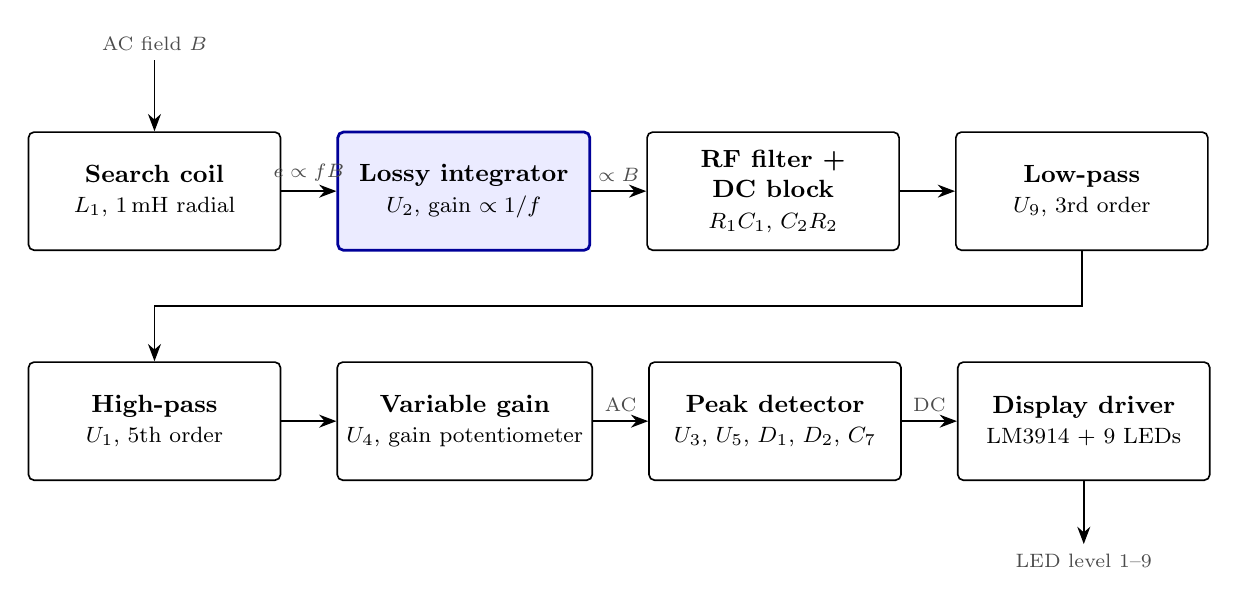
\begin{tikzpicture}[
      node distance=6mm and 7mm,
      blk/.style={draw, rounded corners=2pt, align=center, minimum width=32mm,
                  minimum height=15mm, font=\small, line width=0.6pt},
      key/.style={blk, fill=blue!8, draw=blue!60!black, line width=1pt},
      sig/.style={-{Stealth[length=2.2mm]}, line width=0.6pt},
      lab/.style={font=\scriptsize, text=black!70}]
    % row 1
    \node[blk] (coil) {\textbf{Search coil}\\ \footnotesize $L_1$, \SI{1}{\milli\henry} radial};
    \node[key, right=of coil] (int) {\textbf{Lossy integrator}\\ \footnotesize $U_2$, gain $\propto 1/f$};
    \node[blk, right=of int] (rfdc) {\textbf{RF filter +}\\ \textbf{DC block}\\ \footnotesize $R_1C_1$, $C_2R_2$};
    \node[blk, right=of rfdc] (lpf) {\textbf{Low-pass}\\ \footnotesize $U_9$, 3rd order};
    % row 2
    \node[blk, below=14mm of coil] (hpf) {\textbf{High-pass}\\ \footnotesize $U_1$, 5th order};
    \node[blk, right=of hpf] (gain) {\textbf{Variable gain}\\ \footnotesize $U_4$, gain potentiometer};
    \node[blk, right=of gain] (pk) {\textbf{Peak detector}\\ \footnotesize $U_3$, $U_5$, $D_1$, $D_2$, $C_7$};
    \node[blk, right=of pk] (disp) {\textbf{Display driver}\\ \footnotesize LM3914 + 9 LEDs};
    % input and output
    \draw[sig] ([yshift=9mm]coil.north) node[above, lab] {AC field $B$} -- (coil.north);
    \draw[sig] (disp.south) -- ++(0,-8mm) node[below, lab] {LED level 1--9};
    % signal path
    \draw[sig] (coil) -- node[above, lab] {$e\propto fB$} (int);
    \draw[sig] (int)  -- node[above, lab] {$\propto B$} (rfdc);
    \draw[sig] (rfdc) -- (lpf);
    \draw[sig] (lpf.south) -- ++(0,-7mm) -| (hpf.north);
    \draw[sig] (hpf)  -- (gain);
    \draw[sig] (gain) -- node[above, lab] {AC} (pk);
    \draw[sig] (pk)   -- node[above, lab] {DC} (disp);
  \end{tikzpicture}}
  \caption{Top-level block diagram. The integrator (shaded) cancels the
           coil's rise in output with frequency.}
  \label{fig:arch-block}
\end{figure}

\begin{table}[htbp]
  \centering
  \caption{Stages of the signal chain.}
  \label{tab:arch-stages}
  \small
  \begin{tabular}{@{}llll@{}}
    \toprule
    Stage & Main parts & Function & Key parameter \\
    \midrule
    Search coil      & $L_1$ & Field to EMF & $\hat e = 2\pi f N A \hat B$ \\
    Lossy integrator & $U_2$, $R_{14}$, $C_{22}$, $R_{23}$ & Frequency compensation & $R_{14}C_{22} = \SI{10}{\micro\second}$ \\
    RF filter        & $R_1$, $C_1$ & Remove RF & \SI{339}{\kilo\hertz} \\
    DC block         & $C_2$, $R_2$ & Remove integrator offset & \SI{0.72}{\hertz} \\
    Low-pass         & $U_9$, $R_3$--$R_7$, $C_3$--$C_5$ & Reject RF and noise & \SI{241}{\kilo\hertz}, $\times1.589$ \\
    High-pass        & $U_1$, $C_8$--$C_{12}$ & Lower band limit & \SI{18.1}{\hertz}, $\times1.589$ \\
    Variable gain    & $U_4$, $R_8$, $R_9$ & Gain adjustment & $\times2$ (reference) \\
    Peak detector    & $U_3$, $U_5$, $D_1$, $D_2$, $C_7$, $R_{21}$ & AC to DC peak & $\tau = \SI{39}{\milli\second}$ \\
    Display driver   & LM3914, $R_{19}$, $R_{20}$, trimpots & Level to LED & 10 equal steps \\
    \bottomrule
  \end{tabular}
\end{table}

% ---------------------------------------------------------------------
\subsection{Signal Chain}
\label{sec:arch-stages}

\subsubsection{Search Coil}
Two options were considered for the sensing element: winding a coil by hand, or using a ready-made one. Irregularities in a hand-wound coil, such as uneven winding and an uncertain number of turns, would reduce the repeatability of the device. A radial inductor has the same structure as a search coil and is made to a consistent specification, so an off-the-shelf \SI{1}{\milli\henry} radial inductor ($L_1$), housed in the probe, was used as the sensing element. By Faraday's law~\cite{tumanski2007}, a sinusoidal field of peak amplitude $\hat B$ and frequency $f$ directed along the coil axis induces an EMF of peak amplitude
\begin{equation}
  \hat e = 2\pi f\,N A\,\hat B,
  \label{eq:emf}
\end{equation}
where $N$ is the number of turns and $A$ is the effective area of the coil. The ferrite drum core of the inductor concentrates the flux, so that $A$ exceeds the geometric area of the winding.

A radial inductor was chosen because it is readily available and provides sufficient EMF at \SI{50}{\hertz}. The coil responds only to the component of the field along its axis, so the reading varies with the angle between the probe and the field. Together with the input resistor $R_{14}$ of the integrator stage, the coil inductance forms a pole at $R_{14}/(2\pi L_1) = \SI{15.9}{\kilo\hertz}$, which sets the upper limit of the operating band. This limit could be raised by increasing $R_{14}$. However, $R_{14}$ also sets the integrator gain through $R_{14}C_{22}$ and its DC gain through $R_{23}/R_{14}$, so $C_{22}$ and $R_{23}$ would have to be scaled with it.

\subsubsection{Lossy Integrator (Pre-amplifier)}
From the circuit schematic (Figure~\ref{fig:ltspice_schematic}), the integrator~\cite{horowitz2015} has the following transfer function:
\begin{equation}
  H_{\mathrm{int}}(s) = -\frac{R_{23}}{R_{14}}\cdot\frac{1}{1 + sR_{23}C_{22}}
  \;\approx\; -\frac{1}{sR_{14}C_{22}} \quad \text{for } f \gg \frac{1}{2\pi R_{23}C_{22}}.
  \label{eq:integ}
\end{equation}
Above the corner frequency $1/(2\pi R_{23}C_{22}) = \SI{3.98}{\hertz}$, the gain falls in inverse proportion to frequency. Multiplying \eqref{eq:emf} by the magnitude of \eqref{eq:integ} gives an output amplitude of $N A \hat B/(R_{14}C_{22})$, which is independent of frequency. Therefore, the output is proportional to the field strength alone.

The integrator is described as lossy because $R_{23}$ (\SI{400}{\kilo\ohm}) limits its DC gain to $-R_{23}/R_{14} = -4000$. Without $R_{23}$, the input offset voltage and bias current of the op-amp would be integrated continuously and the output would drift to a supply rail.

\subsubsection{RF Filter and DC Block}
The integrator output first passes through a first-order low-pass filter formed by $R_1$ (\SI{100}{\ohm}) and $C_1$ (\SI{4.7}{\nano\farad}), with a cut-off frequency of \SI{339}{\kilo\hertz}. This filter attenuates RF signals picked up by the probe and cable, and $R_1$ isolates the integrator output from the capacitive load of $C_1$. A high-pass network formed by $C_2$ (\SI{10}{\micro\farad}) and $R_2$ (\SI{22}{\kilo\ohm}), with a cut-off frequency of \SI{0.72}{\hertz}, then blocks the DC offset of the integrator. A non-polarized capacitor is used for $C_2$ because the polarity of this offset could be positive or negative. $R_2$ also provides the DC bias path for the op-amp in the subsequent non-inverting amplifier.

\subsubsection{Low-Pass Filter}
The low-pass filter is a third-order design consisting of a passive RC pair ($R_3$, $C_3$) followed by a Sallen--Key configuration~\cite{karki2002} built around $U_9$ ($R_4$, $R_5$, $C_4$, $C_5$). With $R = \SI{2.7}{\kilo\ohm}$ and $C = \SI{150}{\pico\farad}$, the natural frequency of the Sallen--Key section is \SI{393}{\kilo\hertz}. Combined with the preceding RC filter and its loading, the stage has a passband gain of 1.589 and a \SI{-3}{\deci\bel} frequency of \SI{241}{\kilo\hertz}.

Since the upper edge of the operating band is already set by the search coil at \SI{15.9}{\kilo\hertz}, the purpose of this filter is to reject radio-frequency interference, such as broadcast signals and switching-supply noise.

\subsubsection{High-Pass Filter}
The high-pass filter is a fifth-order design consisting of three passive RC sections ($C_8$--$C_{10}$ with $R_{15}$, $R_{16}$ and $R_{10}$), each with a corner frequency of \SI{4.08}{\hertz}, followed by a Sallen--Key high-pass section~\cite{karki2002} built around $U_1$ ($C_{11}$, $C_{12}$, $R_{22}$, $R_{11}$). The Sallen--Key section has a natural frequency of \SI{8.76}{\hertz} and a quality factor of 1.45. On its own, this section would produce a peak in the response near its natural frequency. Combined with the gradual roll-off of the three passive sections, however, it yields a flat passband with a \SI{-3}{\deci\bel} frequency of \SI{18.1}{\hertz}.

This filter rejects $1/f$ noise, slow drift and the low-frequency EMF induced when the probe is moved through the Earth's static magnetic field, while passing mains-frequency fields with negligible loss.

\subsubsection{Variable Gain Stage}
The variable gain stage ($U_4$) is a non-inverting amplifier with a gain of
\begin{equation}
  G = 1 + \frac{R_9}{R_8}.
  \label{eq:gain}
\end{equation}
The resistance $R_9$ is adjusted by the user through the gain potentiometer on the enclosure, which allows one of three field strength ranges to be mapped to the full range of the output LEDs. The three settings are marked on a label around the knob: \SIrange{5}{25}{\micro\tesla}, \SIrange{10}{40}{\micro\tesla} and \SIrange{20}{90}{\micro\tesla}.

\subsubsection{Precision Peak Detector}
The precision peak detector~\cite{horowitz2015,ti_an31} converts the AC signal into a DC voltage equal to its positive peak. Op-amp $U_3$ and diode $D_1$ form a superdiode that charges the hold capacitor $C_7$ (\SI{0.1}{\micro\farad}), and the voltage follower $U_5$ buffers $C_7$ and returns its voltage to the inverting input of $U_3$ through $R_{18}$. Because $D_1$ lies inside this feedback loop, $U_3$ drives $C_7$ until the capacitor voltage equals the input voltage, and the forward voltage of the diode introduces no error. $R_{17}$ matches $R_{18}$, so that both inputs of $U_3$ see equal source resistances.

The held voltage decays through $R_{21}$ (\SI{390}{\kilo\ohm}) with a time constant $\tau = R_{21}C_7 = \SI{39}{\milli\second}$, which allows the display to follow a decreasing field.

\subsubsection{Display Driver}
The LM3914 display driver~\cite{ti_lm3914} compares the held voltage with the taps of an internal ladder of ten equal resistors connected between its RLO and RHI pins. The voltages at the two ends of the ladder, $V_{\mathrm{RLO}}$ and $V_{\mathrm{RHI}}$, are set by the reference network ($R_{19}$, $R_{20}$) and two multiturn trimpots, which are adjusted during calibration. Nine of the ten outputs are used, and output 1 is left unconnected because, in dot mode, it sinks a small current continuously. LED $k$ therefore lights when the held voltage exceeds
\begin{equation}
  V_k = V_{\mathrm{RLO}} + \frac{(k+1)\,(V_{\mathrm{RHI}} - V_{\mathrm{RLO}})}{10},
  \qquad k = 1, \dots, 9,
  \label{eq:vk}
\end{equation}
so the thresholds are equally spaced. The nine LEDs form three color bands: green (LEDs 1--3), yellow (LEDs 4--6) and red (LEDs 7--9). The driver operates in dot mode, in which only the LED corresponding to the present level is lit. This minimizes both the supply current and the power dissipated in the driver. Since the LM3914 regulates the current of each output at approximately ten times the current drawn from its reference output, no series resistors are required for the LEDs.

\subsubsection{Power Supply}
Two \SI{9}{\volt} batteries with one terminal connected to the opposite terminal of the other are used to build the dual supply required. The dual supply allows the AC signal to swing symmetrically about ground through the integrator, filter and gain stages without any biasing network. The six TL071 op-amps~\cite{ti_tl07x} draw from both rails, whereas the LM3914 and the LEDs operate between ground and the positive rail. The current drawn from the positive rail is estimated at about \SI{28}{\milli\ampere} with one LED lit: approximately \SI{8.4}{\milli\ampere} for the op-amps, a few milliamperes of quiescent current for the LM3914 and about \SI{16}{\milli\ampere} for the LED. The negative rail supplies about \SI{24}{\milli\ampere}, including the continuously lit power indication LED. This wiring allows a more balanced draining of the two batteries. A power switch on the enclosure turns the detector on and off.

% ---------------------------------------------------------------------
\subsection{Gain and Signal-Level Budget}
\label{sec:arch-budget}

Table~\ref{tab:arch-budget} traces the gain and signal amplitude through the chain for a field that induces \SI{40}{\milli\volt} in the coil at \SI{1}{\kilo\hertz}, and for a field of the same strength at \SI{50}{\hertz}, which induces only \SI{2}{\milli\volt}. Although the two EMFs differ by a factor of 20, the integrator gains differ by the same factor in the opposite direction. Both signals therefore reach almost the same amplitude at the integrator output and the same DC level at the peak detector, and they light the same LED. The largest signal occurs at the output of the variable gain stage, which is therefore the first point to clip, at approximately $\pm\SI{7.5}{\volt}$ with $\pm\SI{9}{\volt}$ supplies.

\begin{table}[htbp]
  \centering
  \caption{Gain and signal level at each stage output for the same field
           at \SI{50}{\hertz} and \SI{1}{\kilo\hertz} (gain stage $\times2$).}
  \label{tab:arch-budget}
  \small
  \begin{tabular}{@{}lrrrr@{}}
    \toprule
    & \multicolumn{2}{c}{Gain (V/V)} & \multicolumn{2}{c}{Level (peak)} \\
    \cmidrule(lr){2-3}\cmidrule(l){4-5}
    Stage output & \SI{50}{\hertz} & \SI{1}{\kilo\hertz} & \SI{50}{\hertz} & \SI{1}{\kilo\hertz} \\
    \midrule
    Coil EMF (input)         & --   & --   & \SI{2}{\milli\volt} & \SI{40}{\milli\volt} \\
    Lossy integrator         & 315  & 15.8 & \SI{0.63}{\volt} & \SI{0.63}{\volt} \\
    RF/DC block + low-pass   & 1.58 & 1.58 & \SI{1.00}{\volt} & \SI{1.00}{\volt} \\
    High-pass                & 1.56 & 1.59 & \SI{1.56}{\volt} & \SI{1.59}{\volt} \\
    Variable gain            & 2    & 2    & \SI{3.12}{\volt} & \SI{3.18}{\volt} \\
    Peak detector (DC)       & 1    & 1    & \SI{3.12}{\volt} & \SI{3.18}{\volt} \\
    \midrule
    Total, EMF to peak detector & 1559 & 79.5 & \multicolumn{2}{c}{Same LED lit} \\
    \bottomrule
  \end{tabular}
\end{table}

% ---------------------------------------------------------------------
\subsection{Frequency-Response Allocation}
\label{sec:arch-freq}

Table~\ref{tab:arch-corners} lists the corner frequencies in the signal chain and the band edge that each one affects, and Figure~\ref{fig:arch-freq} shows the resulting overall response to a field of constant strength. The lower edge of the band is imposed by the fifth-order high-pass filter. The DC block and the integrator corner lie well below it and have no significant effect within the band. The upper edge is defined by the pole formed by the coil inductance and $R_{14}$ at \SI{15.9}{\kilo\hertz}. In simulation, the response to a constant field remains within \SI{3}{\deci\bel} of its \SI{1}{\kilo\hertz} value from \SI{18.6}{\hertz} to \SI{16.0}{\kilo\hertz}, and is only \SI{0.16}{\deci\bel} low at \SI{50}{\hertz}. Hardware testing confirmed a flat response from \SI{50}{\hertz} to \SI{15}{\kilo\hertz}. This range covers mains-frequency fields as well as the higher-frequency fields produced by switch-mode power supplies, fluorescent ballasts and induction cooktops, while excluding the region below \SI{50}{\hertz}, where $1/f$ noise and probe motion become non-negligible.

\begin{table}[htbp]
  \centering
  \caption{Corner frequencies and the band edge each one affects.}
  \label{tab:arch-corners}
  \small
  \begin{tabular}{@{}llr@{}}
    \toprule
    Corner & Set by & Frequency \\
    \midrule
    DC block               & $C_2$, $R_2$           & \SI{0.72}{\hertz} \\
    Integrator lower limit & $R_{23}$, $C_{22}$     & \SI{3.98}{\hertz} \\
    High-pass ($-3$\,dB)   & $C_8$--$C_{12}$, $U_1$ & \SI{18.1}{\hertz} \\
    \midrule
    Coil corner (band top) & $L_1$, $R_{14}$        & \SI{15.9}{\kilo\hertz} \\
    Low-pass ($-3$\,dB)    & $U_9$ stage            & \SI{241}{\kilo\hertz} \\
    RF filter              & $R_1$, $C_1$           & \SI{339}{\kilo\hertz} \\
    \bottomrule
  \end{tabular}
\end{table}

\begin{figure}[htbp]
  \centering
  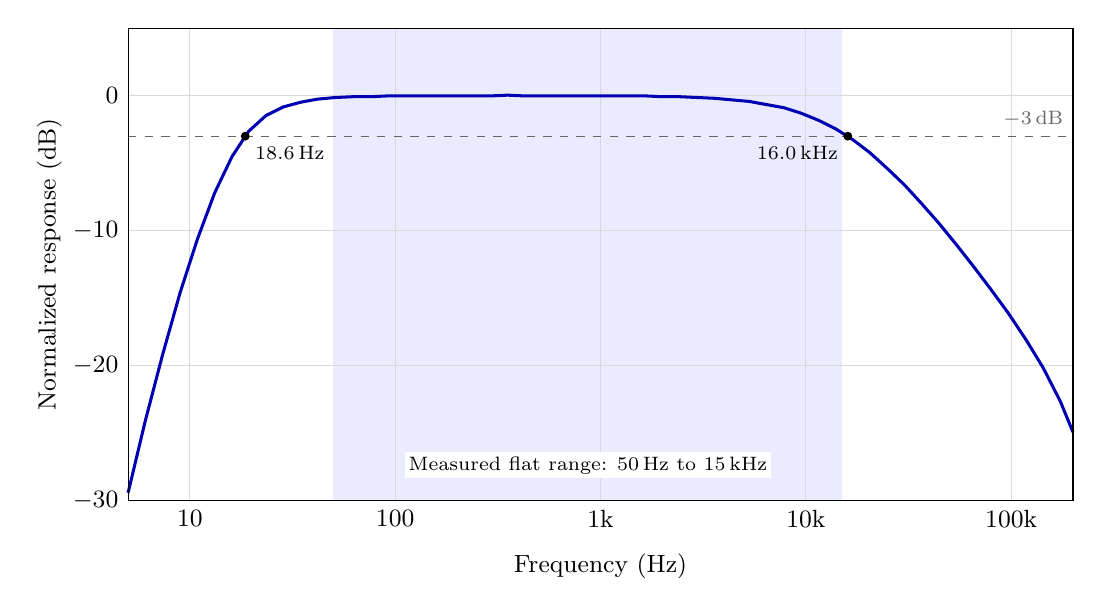
\begin{tikzpicture}[font=\small]
    % measured flat range, 50 Hz to 15 kHz
    \fill[blue!8] (2.608,0) rectangle (9.067,6);
    % grid: decades and 10 dB steps
    \foreach \x in {0.785,3.392,6.0,8.608,11.215} \draw[black!15] (\x,0) -- (\x,6);
    \foreach \y in {1.714,3.429,5.143} \draw[black!15] (0,\y) -- (12,\y);
    % -3 dB reference
    \draw[dashed, black!60] (0,4.629) -- (12,4.629)
      node[above left, font=\scriptsize] {$-3$\,dB};
    % simulated response
    \draw[blue!70!black, line width=1.1pt] plot coordinates {(0.00,0.10) (0.22,1.02) (0.44,1.86) (0.66,2.64) (0.88,3.32) (1.10,3.91) (1.32,4.37) (1.53,4.69) (1.75,4.89) (1.97,5.00) (2.19,5.06) (2.41,5.10) (2.63,5.12) (2.85,5.13) (3.07,5.13) (3.29,5.14) (3.51,5.14) (3.73,5.14) (3.95,5.14) (4.16,5.14) (4.38,5.14) (4.60,5.14) (4.82,5.15) (5.04,5.14) (5.26,5.14) (5.48,5.14) (5.70,5.14) (5.92,5.14) (6.14,5.14) (6.36,5.14) (6.58,5.14) (6.79,5.13) (7.01,5.13) (7.23,5.12) (7.45,5.11) (7.67,5.09) (7.89,5.07) (8.11,5.03) (8.33,4.99) (8.55,4.92) (8.77,4.83) (8.99,4.72) (9.21,4.58) (9.42,4.42) (9.64,4.22) (9.86,4.01) (10.08,3.77) (10.30,3.52) (10.52,3.25) (10.74,2.97) (10.96,2.68) (11.18,2.38) (11.40,2.05) (11.62,1.69) (11.84,1.26) (12.00,0.87)};
    % simulated -3 dB points
    \fill (1.488,4.629) circle (1.6pt) node[below right, font=\scriptsize] {\SI{18.6}{\hertz}};
    \fill (9.14,4.629) circle (1.6pt) node[below left, font=\scriptsize] {\SI{16.0}{\kilo\hertz}};
    \node[font=\scriptsize, fill=white, inner sep=1.5pt] at (5.84,0.45)
      {Measured flat range: \SI{50}{\hertz} to \SI{15}{\kilo\hertz}};
    % frame and axes
    \draw (0,0) rectangle (12,6);
    \foreach \x/\l in {0.785/10, 3.392/100, 6.0/1k, 8.608/10k, 11.215/100k}
      \node[below] at (\x,0) {\l};
    \foreach \y/\l in {0/-30, 1.714/-20, 3.429/-10, 5.143/0}
      \node[left] at (0,\y) {$\l$};
    \node[below] at (6,-0.55) {Frequency (Hz)};
    \node[rotate=90] at (-1.0,3) {Normalized response (dB)};
  \end{tikzpicture}
  \caption{Simulated response to a field of constant strength, normalized to its
           \SI{1}{\kilo\hertz} value. The shaded region is the measured flat range;
           the dots mark the simulated \SI{-3}{\deci\bel} points.}
  \label{fig:arch-freq}
\end{figure}

% ---------------------------------------------------------------------
\subsection{Physical Architecture}
\label{sec:arch-physical}

The electronics are divided between two housings, both 3D-printed in PETG. The probe housing contains the search coil and is connected to the main unit by a coaxial cable, so that the coil can be placed close to a source in confined spaces while the main unit is kept away from it. The main unit holds the PCB and the two batteries in separate compartments, and carries the user interface: the power switch, the gain potentiometer and the nine indicator LEDs. PETG was selected because it is electrically insulating and non-ferromagnetic. Consequently, it does not shield or distort the field being measured.

% ---------------------------------------------------------------------
\subsection{Architectural Alternatives Considered}
\label{sec:arch-alt}

Several alternatives for the sensor and the peak detector were considered during the design. The reasons for rejecting them are summarized in Table~\ref{tab:arch-alt}.

\begin{table}[htbp]
  \centering
  \caption{Alternatives considered.}
  \label{tab:arch-alt}
  \small
  \begin{tabular}{@{}P{0.27\linewidth}P{0.25\linewidth}P{0.40\linewidth}@{}}
    \toprule
    Alternative & Instead of & Why rejected \\
    \midrule
    Hall-effect sensor IC & Radial-inductor search coil & Built for static (DC) fields; a coil captures AC fields better \\
    Passive bridge rectifier & Precision peak detector & Diode drops block about \SI{1.4}{\volt} of signal \\
    Single op-amp + diode peak detector & Two-op-amp precision peak detector & Did not reach the true peak at higher frequencies \\
    \bottomrule
  \end{tabular}
\end{table}

% =====================================================================
% 3. Component Selection
% =====================================================================
\section{Component Selection}
\label{sec:components}

The parts were chosen to be able to run from a $\pm\SI{9}{\volt}$ supply and handle the complete bandwidth of operation. Cost and local availability were other considerations. Since the ICs are plugged into through-hole sockets, they can easily be replaced. Table~\ref{tab:components} lists the key components with their important features and the justification for selection.

\begin{table}[htbp]
  \centering
  \caption{Selected components.}
  \label{tab:components}
  \small
  \begin{tabularx}{\textwidth}{@{}l l l >{\raggedright\arraybackslash}X@{}}
    \toprule
    \textbf{Component} & \textbf{Part} & \textbf{Key specification} & \textbf{Reason for choice} \\
    \midrule
    Search coil & 1\,mH radial inductor & Unshielded, ferrite core & High sensitivity in a small probe tip; sets the 15.9\,kHz upper corner with $R_{14}$ \\
    Op-amps & TL071 ($\times 6$)~\cite{ti_tl07x} & JFET input, 13\,V/$\mu$s & Negligible input current with high-value resistors; ample slew rate at 15\,kHz \\
    Display driver & LM3914~\cite{ti_lm3914} & Linear steps, regulated LED current & Equal field steps; one IC drives all nine LEDs \\
    Diodes & 1N4148~\cite{vishay_1n4148} & 4\,ns recovery, low leakage & Fast peak detection without discharging $C_7$ \\
    Trimmers & 20\,k$\Omega$, 25-turn (3296W) & Multiturn & Fine setting of the display end points during calibration \\
    Probe link & Coaxial cable, SMA & Shielded, screw-locking & No field pickup by the cable; stable connection \\
    Power & 2 $\times$ 9\,V batteries & $\pm$9\,V, no converter & No switching noise or stray field near the sensor \\
    \bottomrule
  \end{tabularx}
\end{table}

\newpage

% =====================================================================
% 4. PCB Design
% =====================================================================
\section{PCB Design}
\label{sec:pcb}

\begin{figure}[H]
  \centering
  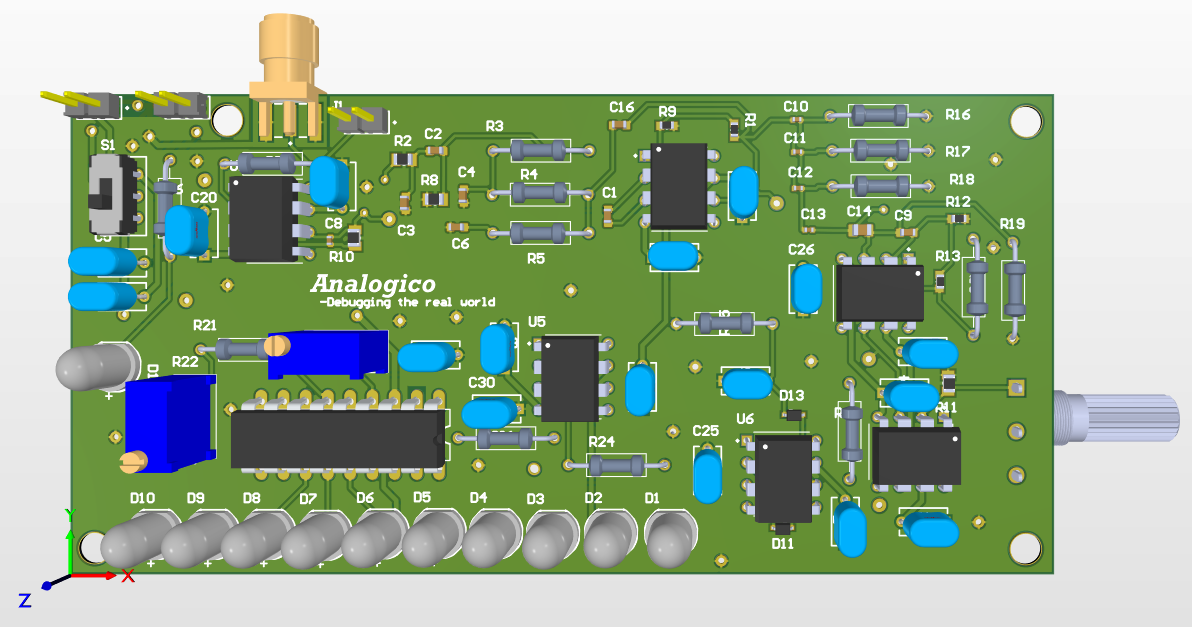
\includegraphics[width=0.9\textwidth]{image1.png}
  \caption{3D render of the PCB.}
  \label{fig:pcb-layout}
\end{figure}

\begin{figure}[H]
  \centering
  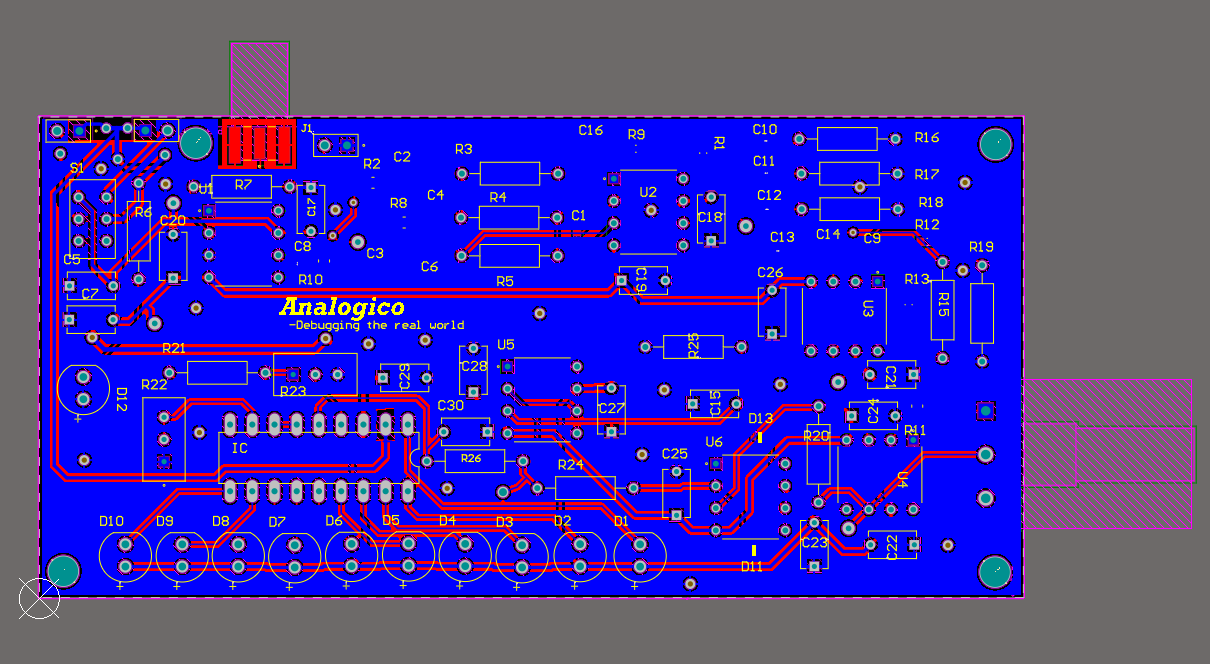
\includegraphics[height=0.24\textwidth]{image3.png}\hfill
  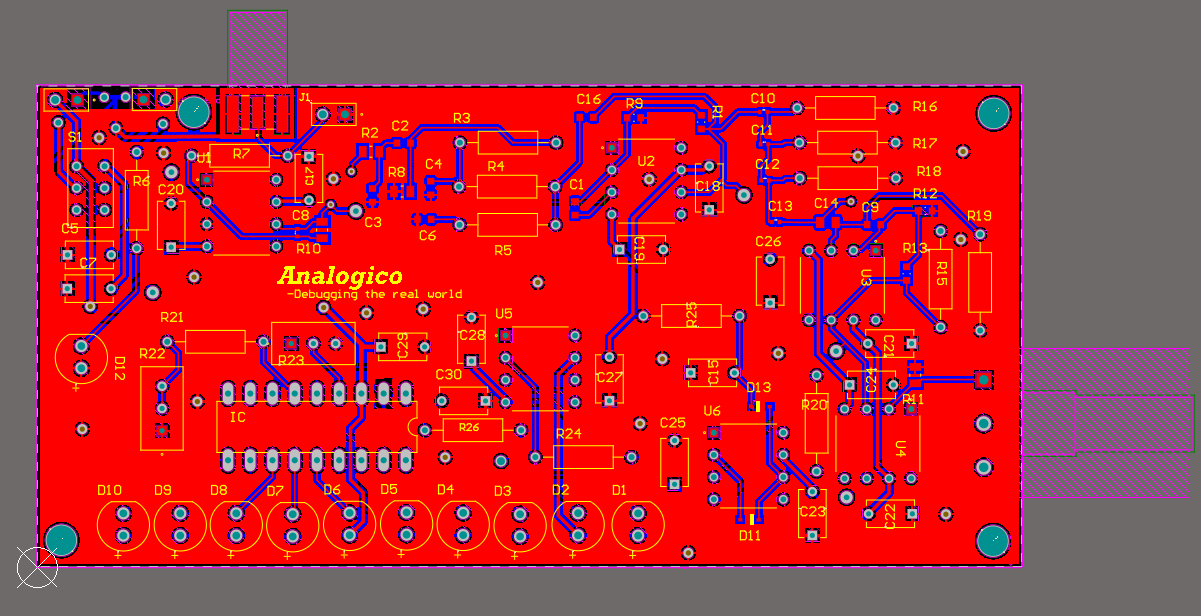
\includegraphics[height=0.24\textwidth]{image2.png}
  \caption{Top (red) and bottom (blue) copper layers.}
  \label{fig:pcb-views}
\end{figure}

The circuit is built on a compact, two-layer PCB combining surface-mount and through-hole components (Figures~\ref{fig:pcb-layout} and~\ref{fig:pcb-views}). It integrates the complete analog signal chain, linking the top coaxial probe connector through the preamplifier, filtering, and peak-detection stages to the bottom-edge 9-LED bar-graph display. Edge-mounted controls, onboard calibration trim potentiometers, test points, and four corner mounting holes simplify tuning and enclosure assembly, while full copper pours on both the top (red) and bottom (blue) layers help shield low-level signals.

\begin{figure}[H]
  \centering
  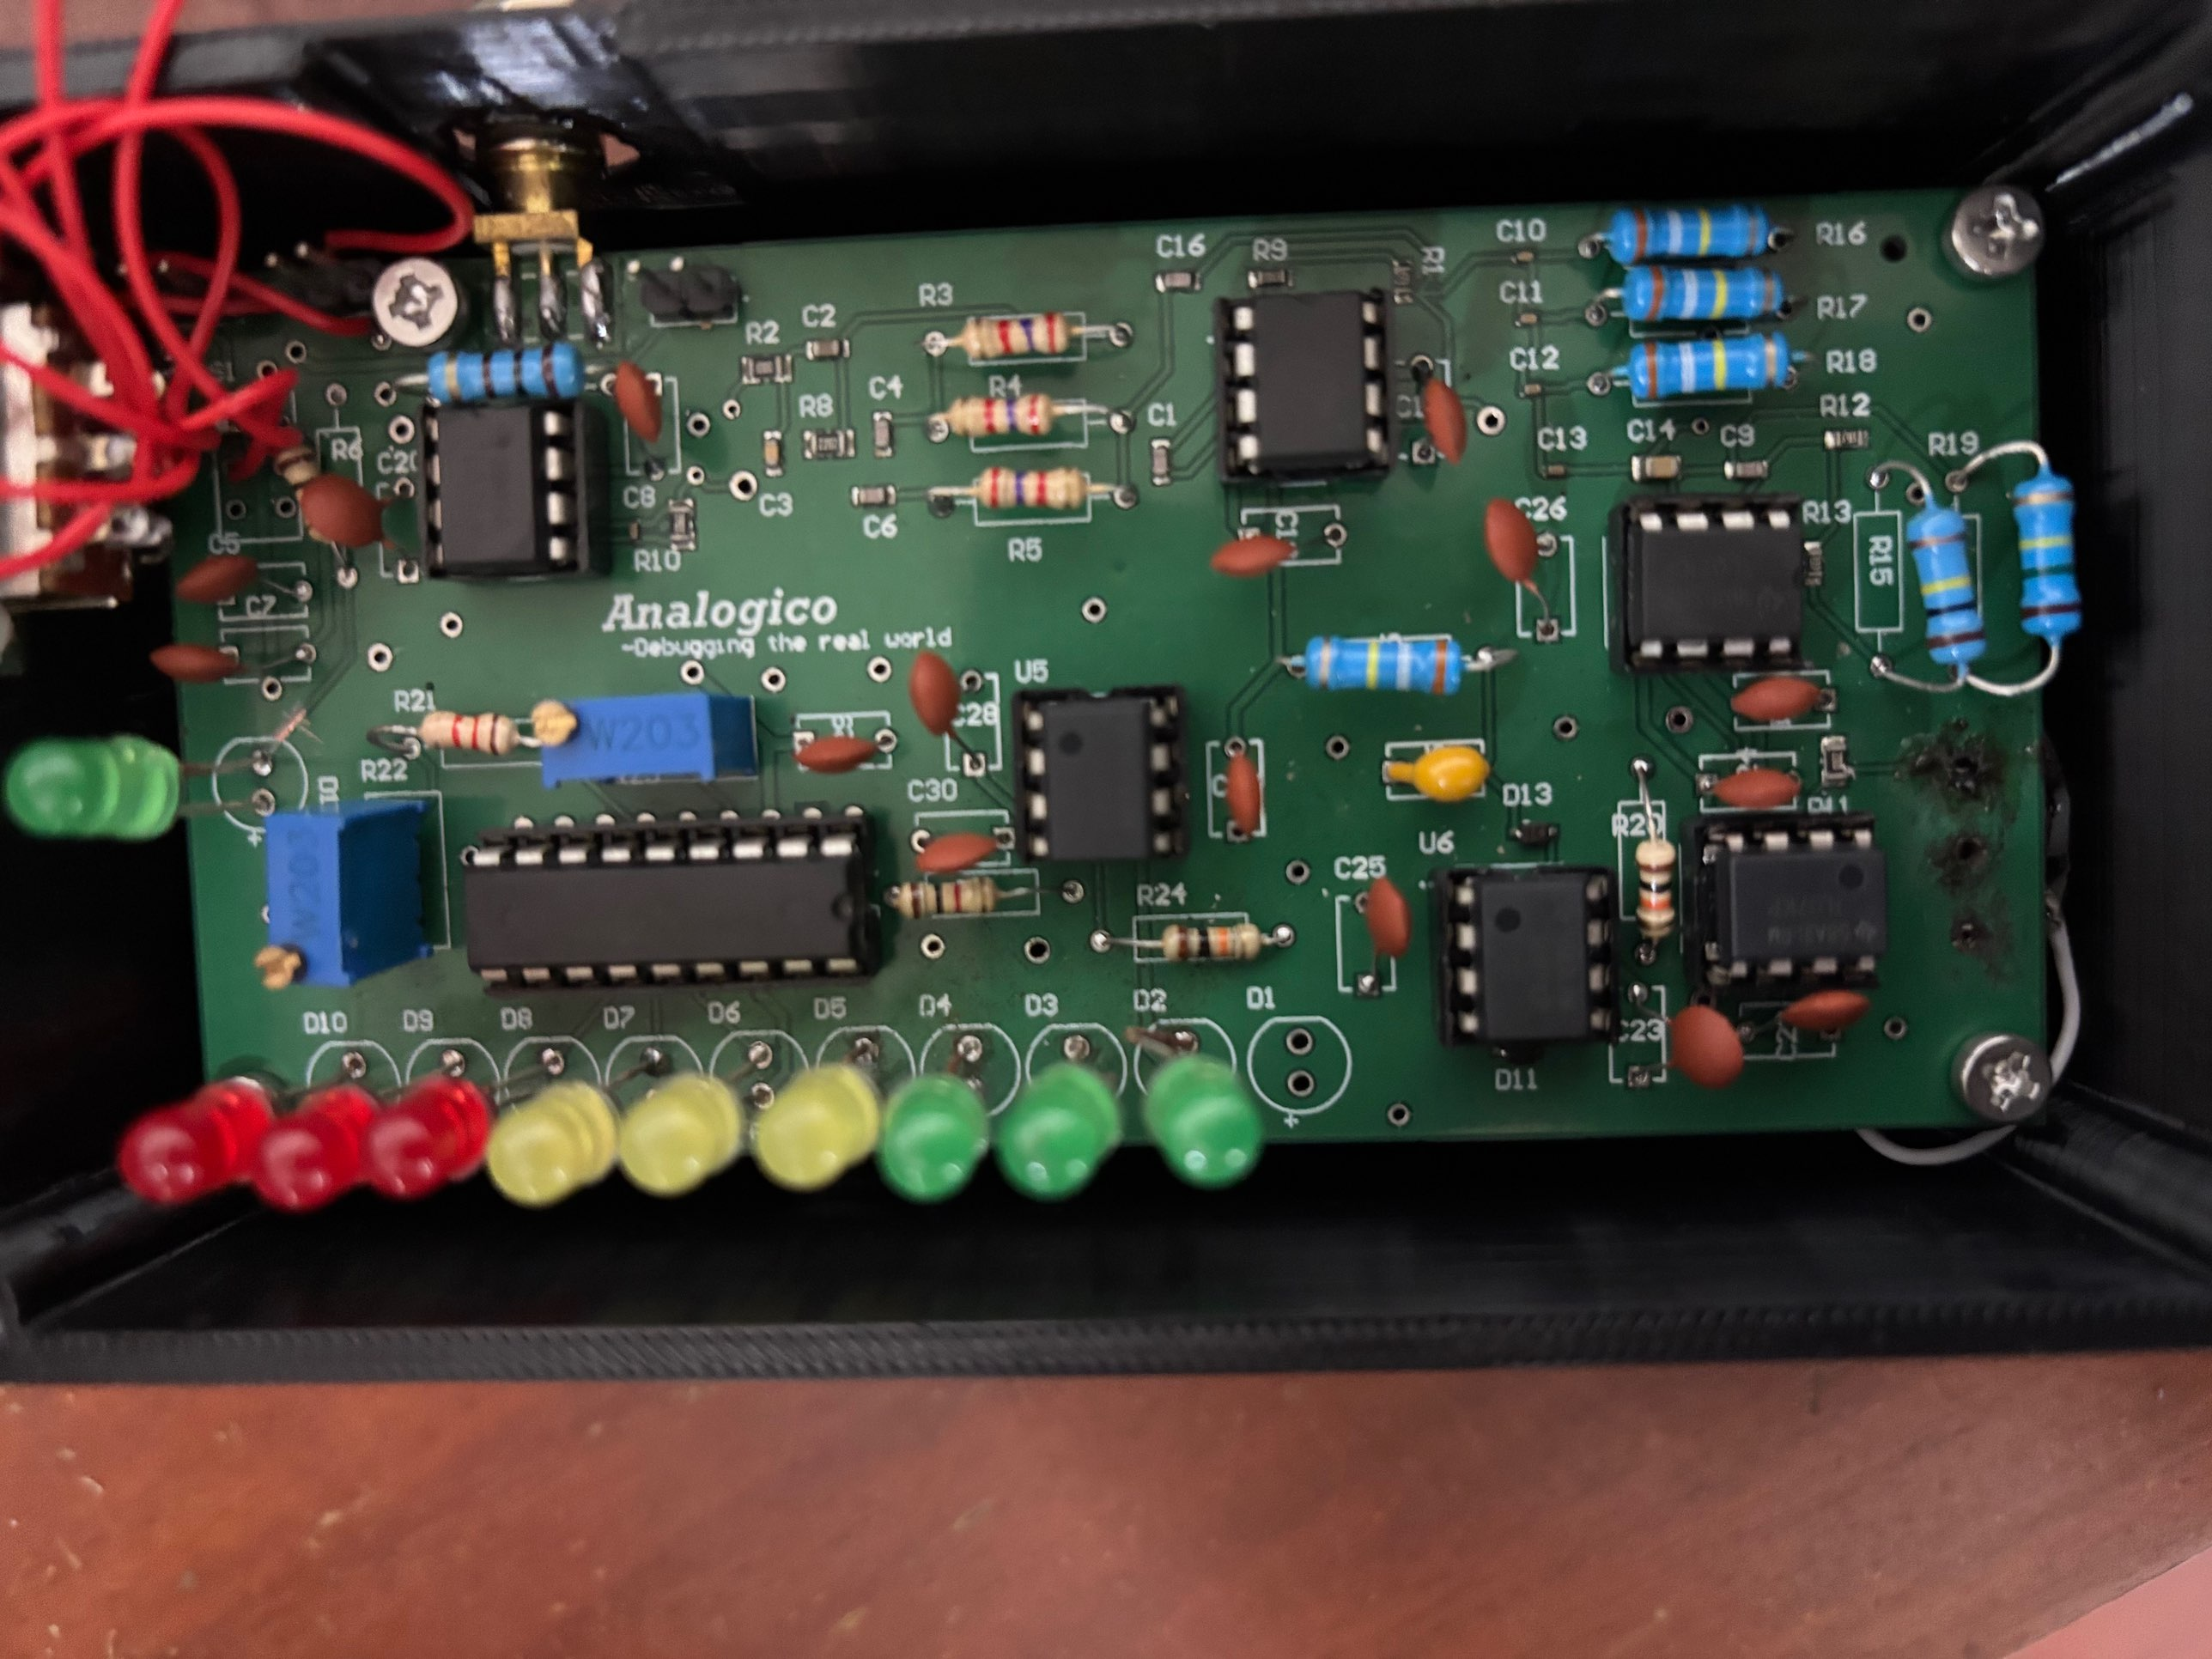
\includegraphics[width=0.9\textwidth]{pcb.jpeg}
  \caption{Assembled PCB mounted inside the enclosure.}
  \label{fig:pcb-installed}
\end{figure}

% =====================================================================
% 5. Enclosure Design
% =====================================================================
\section{Enclosure Design}
\label{sec:enclosure}

The enclosure comprises two components: a probe housing and a main unit. The probe housing contains the radial inductor and a portion of the coaxial cable, while the main unit houses the printed circuit board (PCB) and two \SI{9}{\volt} batteries.

Both components are fabricated using three-dimensional printing with polyethylene terephthalate glycol-modified (PETG). This electrically insulating, non-ferromagnetic material provides mechanical strength without interfering with the alternating magnetic fields being measured.

The probe housing is designed to be compact enough for use in confined spaces while remaining comfortable to hold by hand. The main enclosure is divided into two compartments on opposite sides: one accommodates the PCB, and the other is reserved for the batteries. The probe is connected to the main unit by a coaxial cable. The user interface comprises a power switch, a potentiometer for gain adjustment, and LED indicators. The LEDs are positioned so that their upper portions protrude through the enclosure and remain visible to the user.

\begin{figure}[H]
  \centering
  \begin{minipage}[t]{0.48\linewidth}
    \centering
    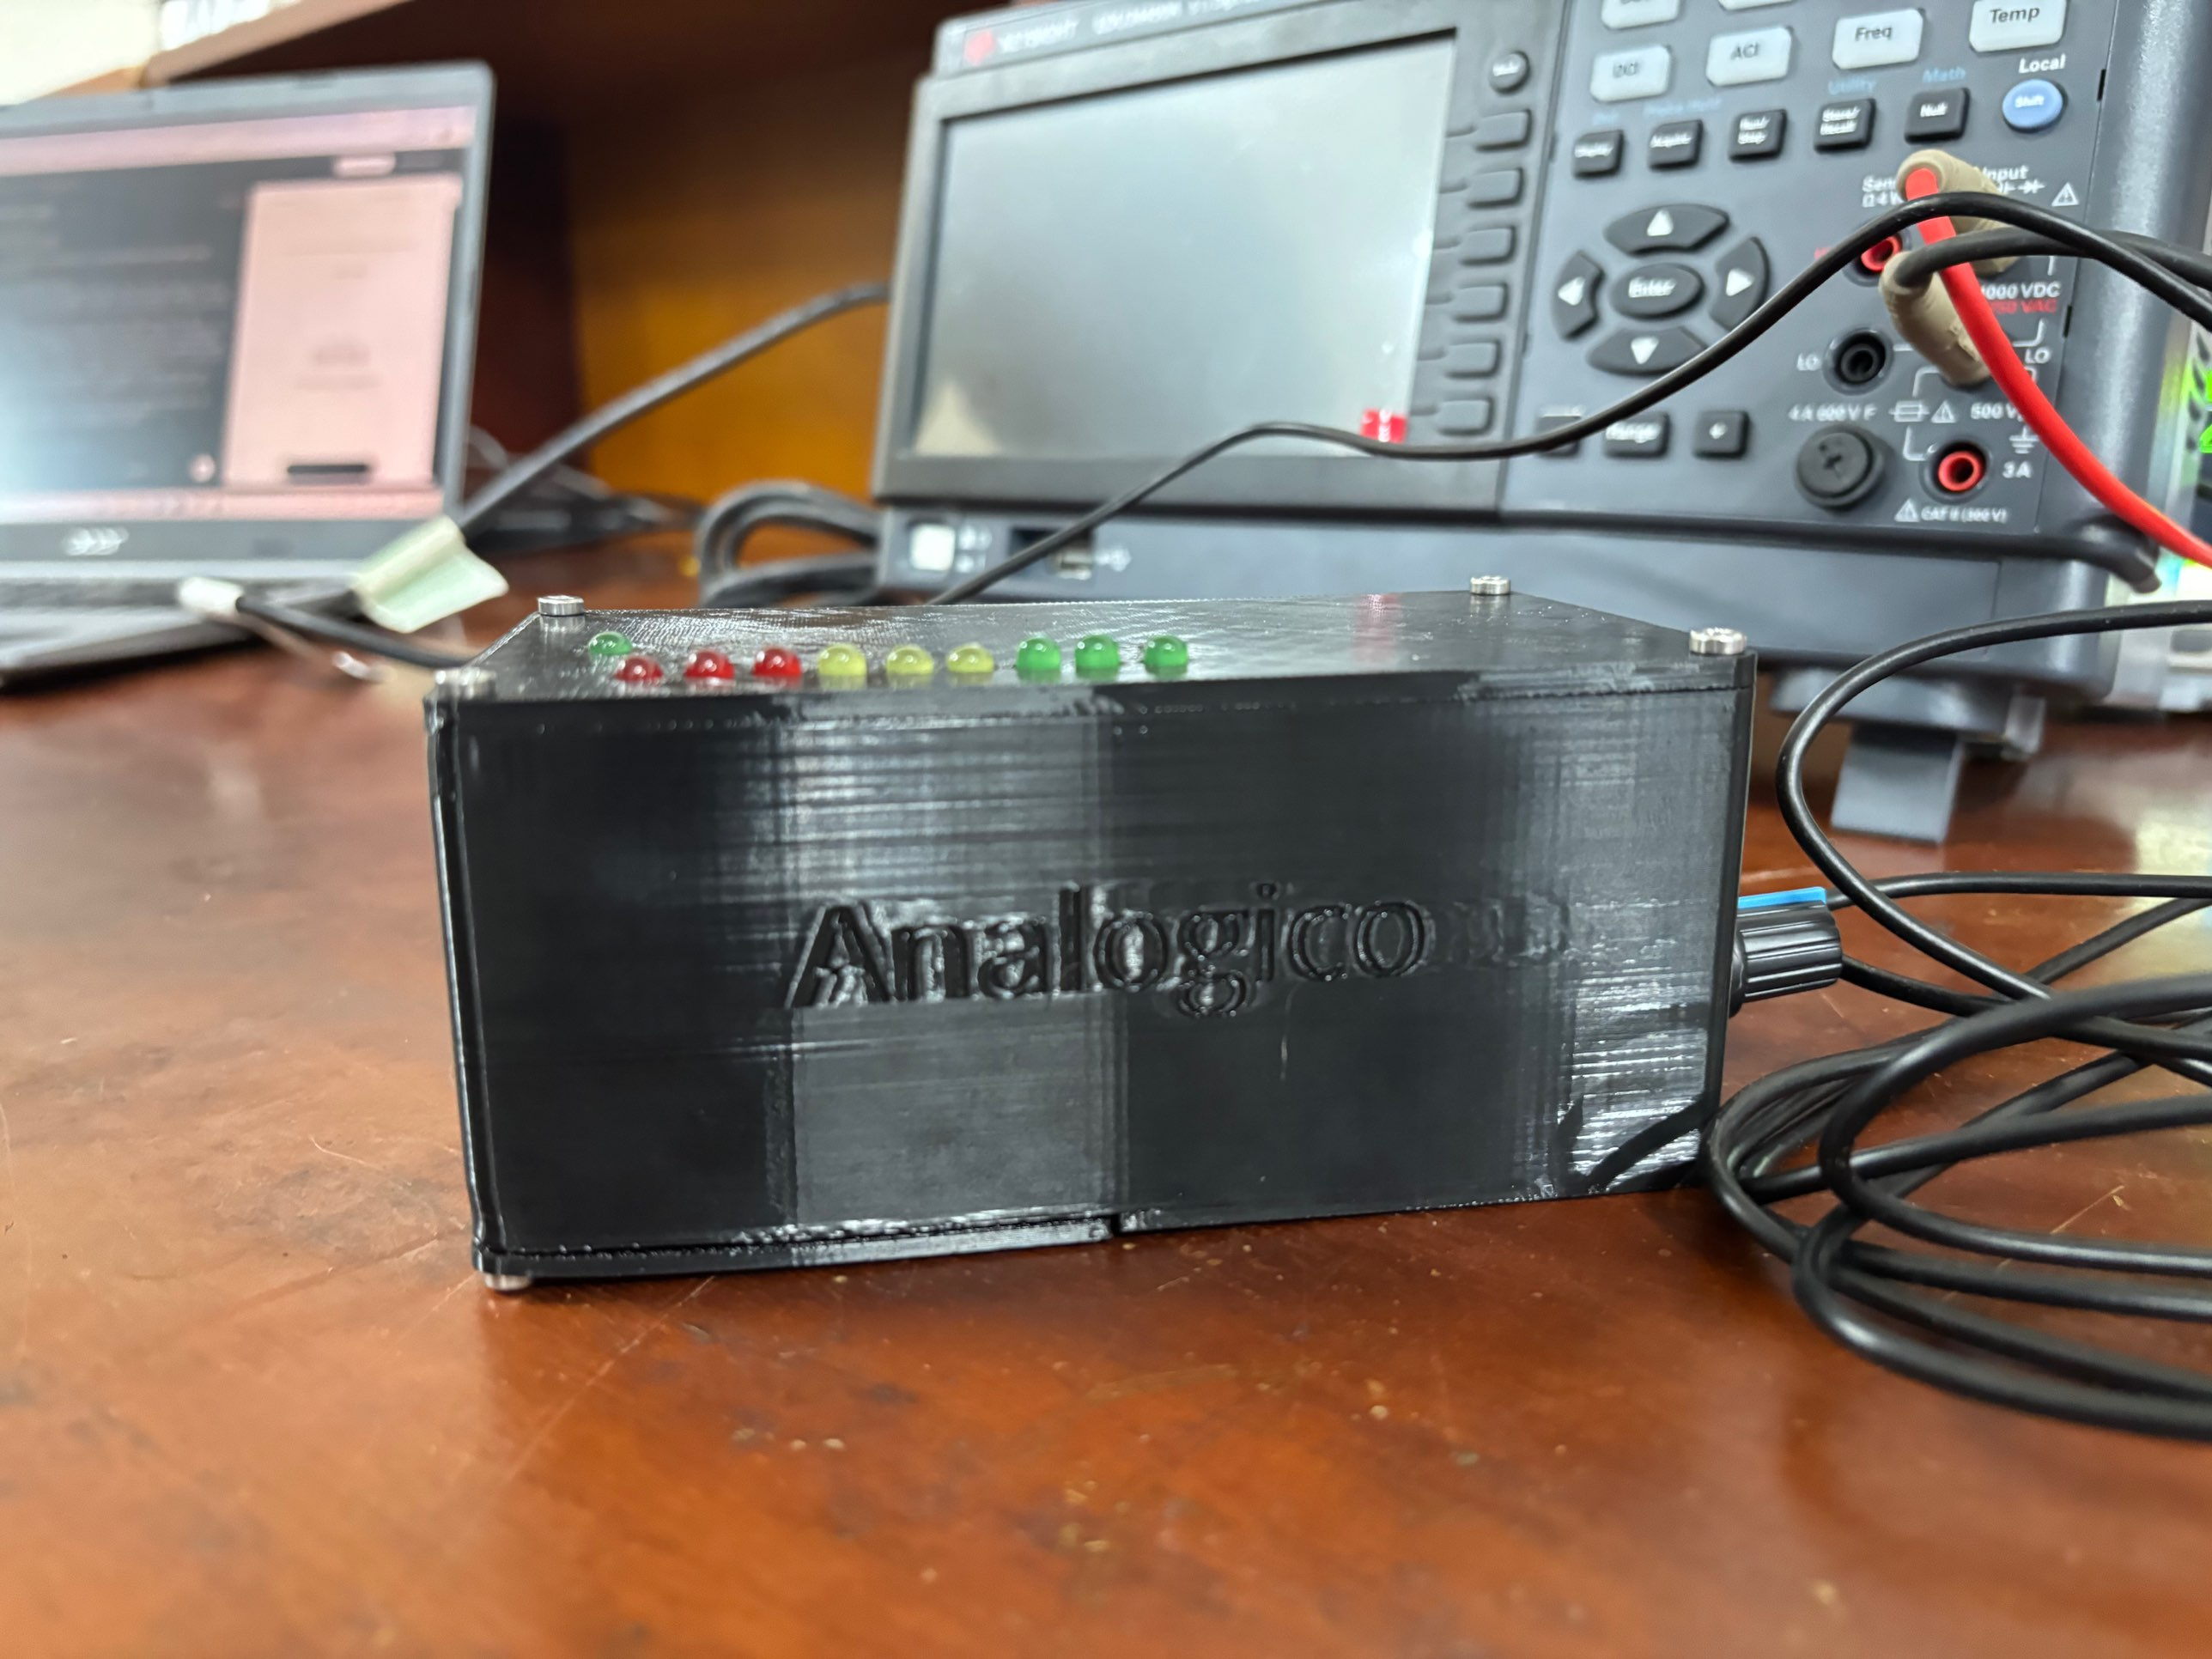
\includegraphics[width=\linewidth,height=4.2cm,keepaspectratio]{enclosure2.jpeg}\\
    {\small Side view with team name}
  \end{minipage}\hfill
  \begin{minipage}[t]{0.48\linewidth}
    \centering
    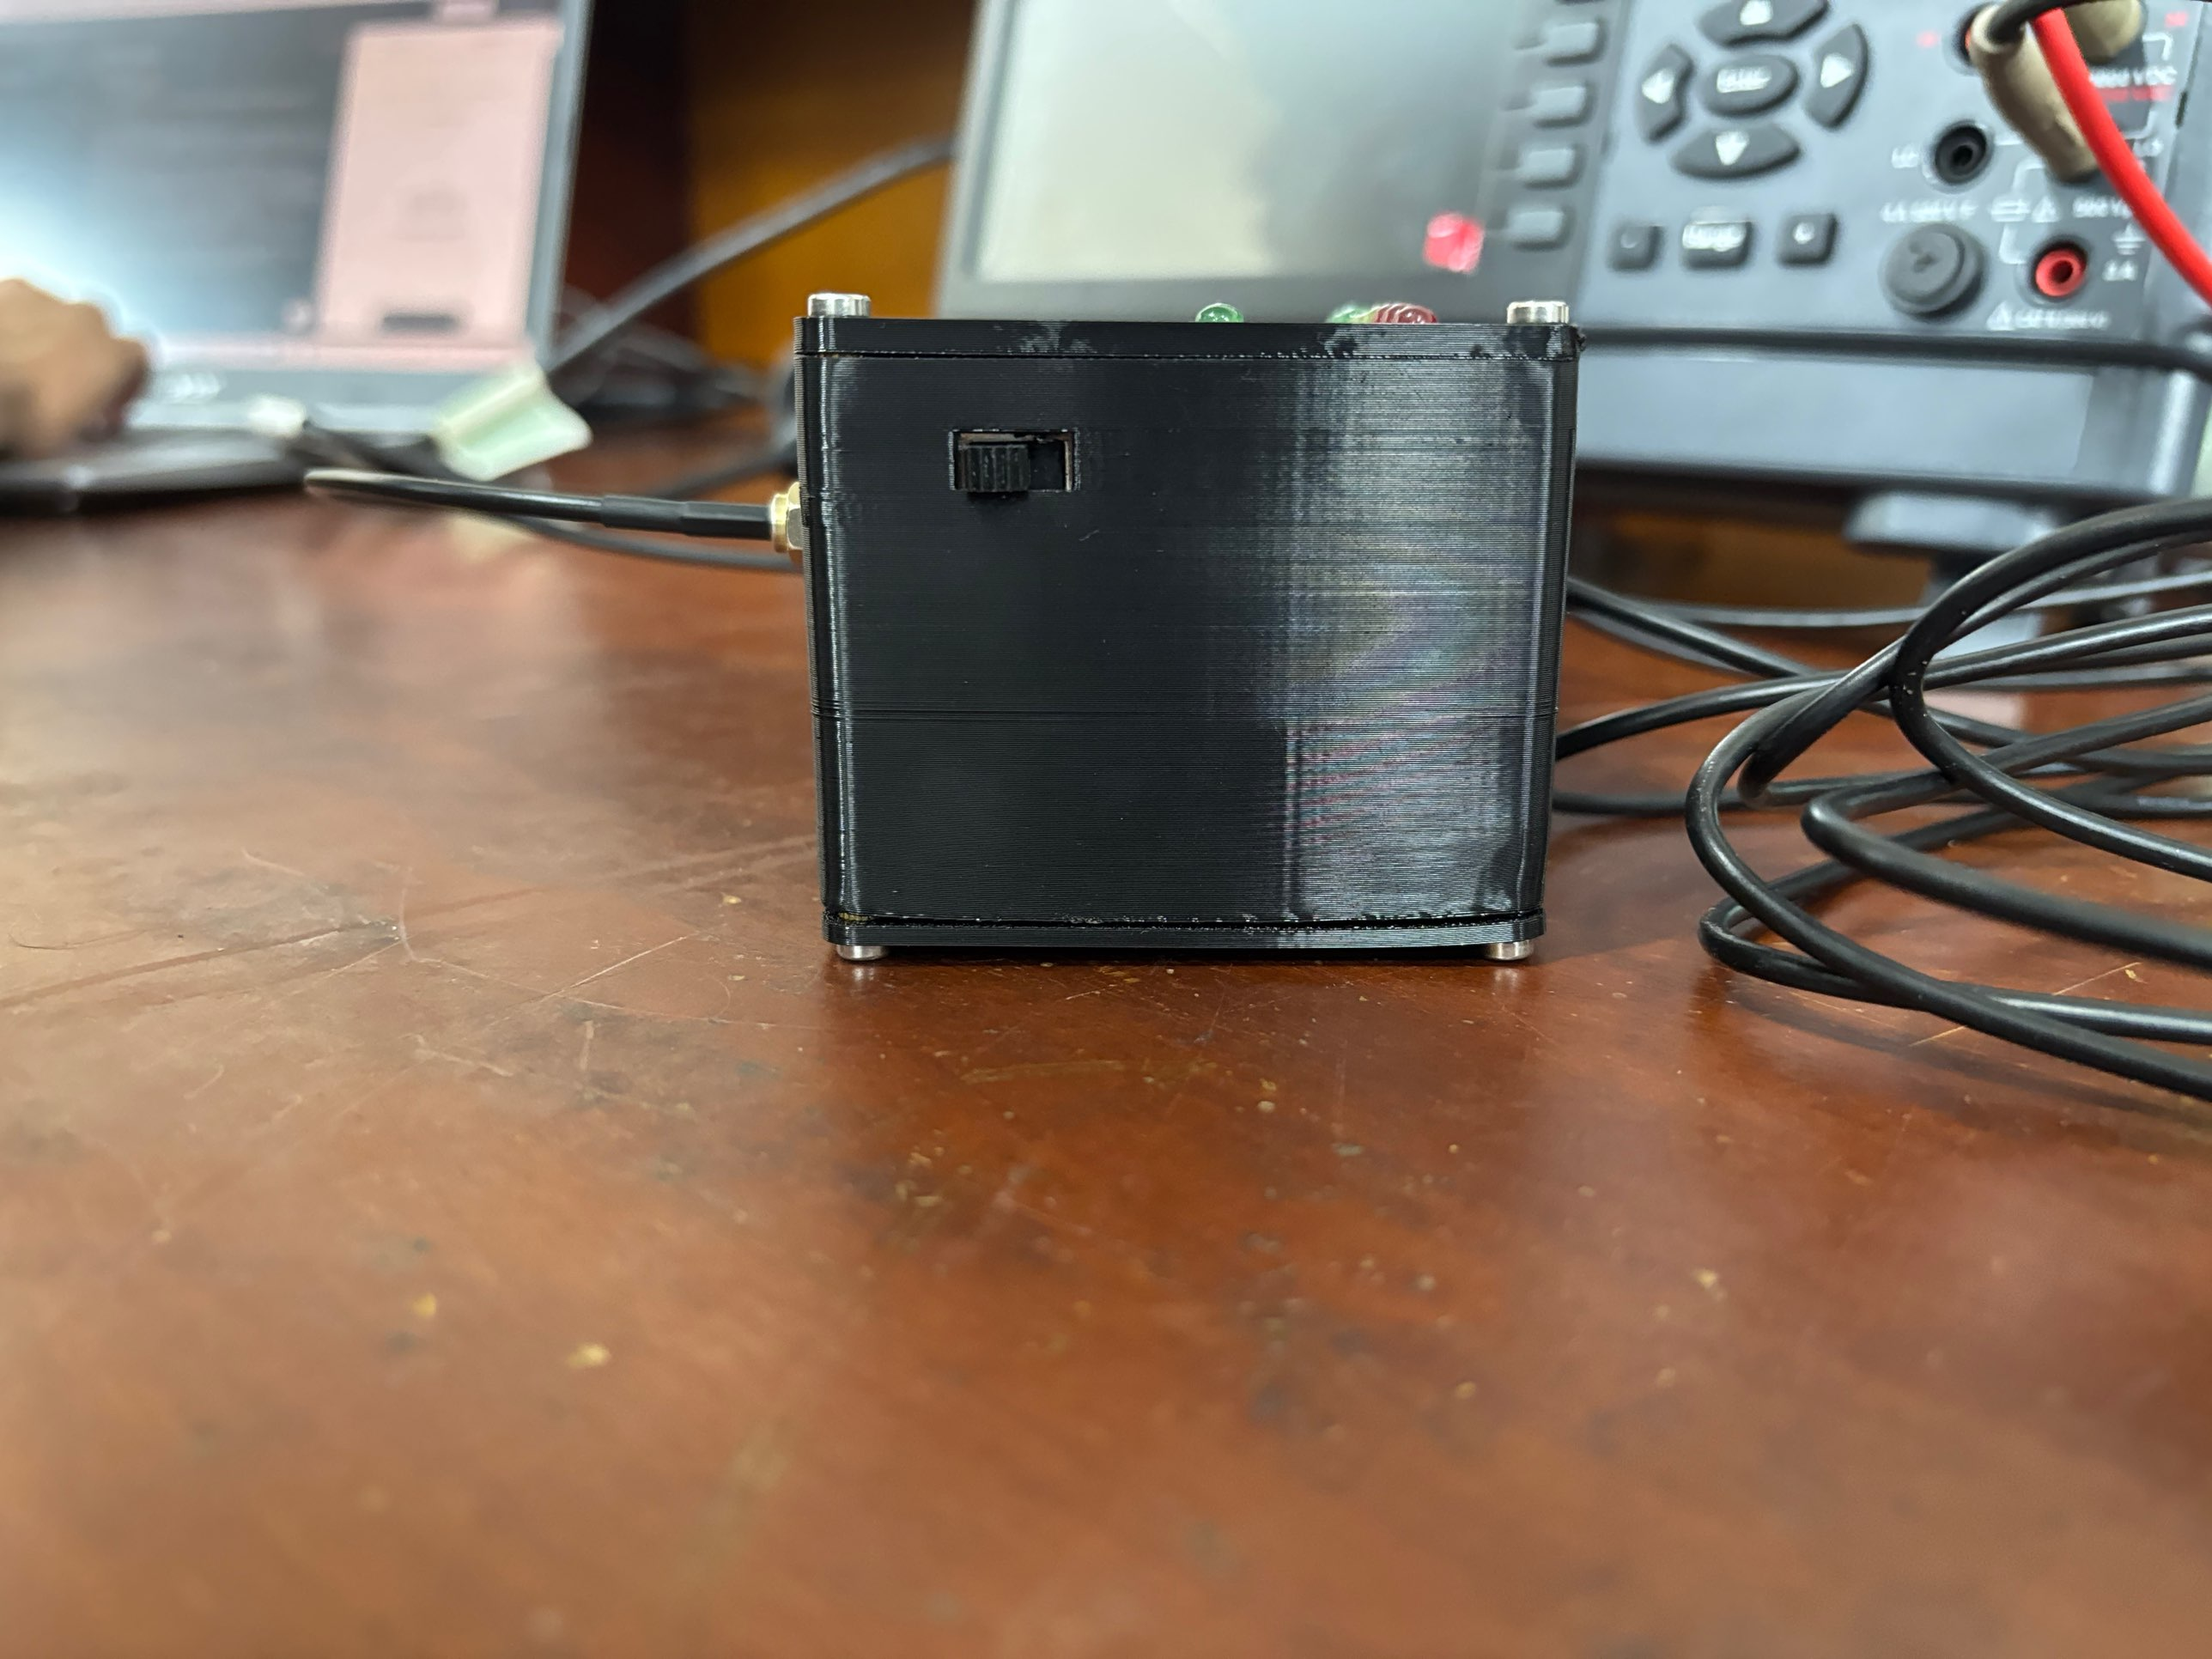
\includegraphics[width=\linewidth,height=4.2cm,keepaspectratio]{enclosure3.jpeg}\\
    {\small Top face and switch}
  \end{minipage}

  \par\medskip
  \begin{minipage}[t]{0.48\linewidth}
    \centering
    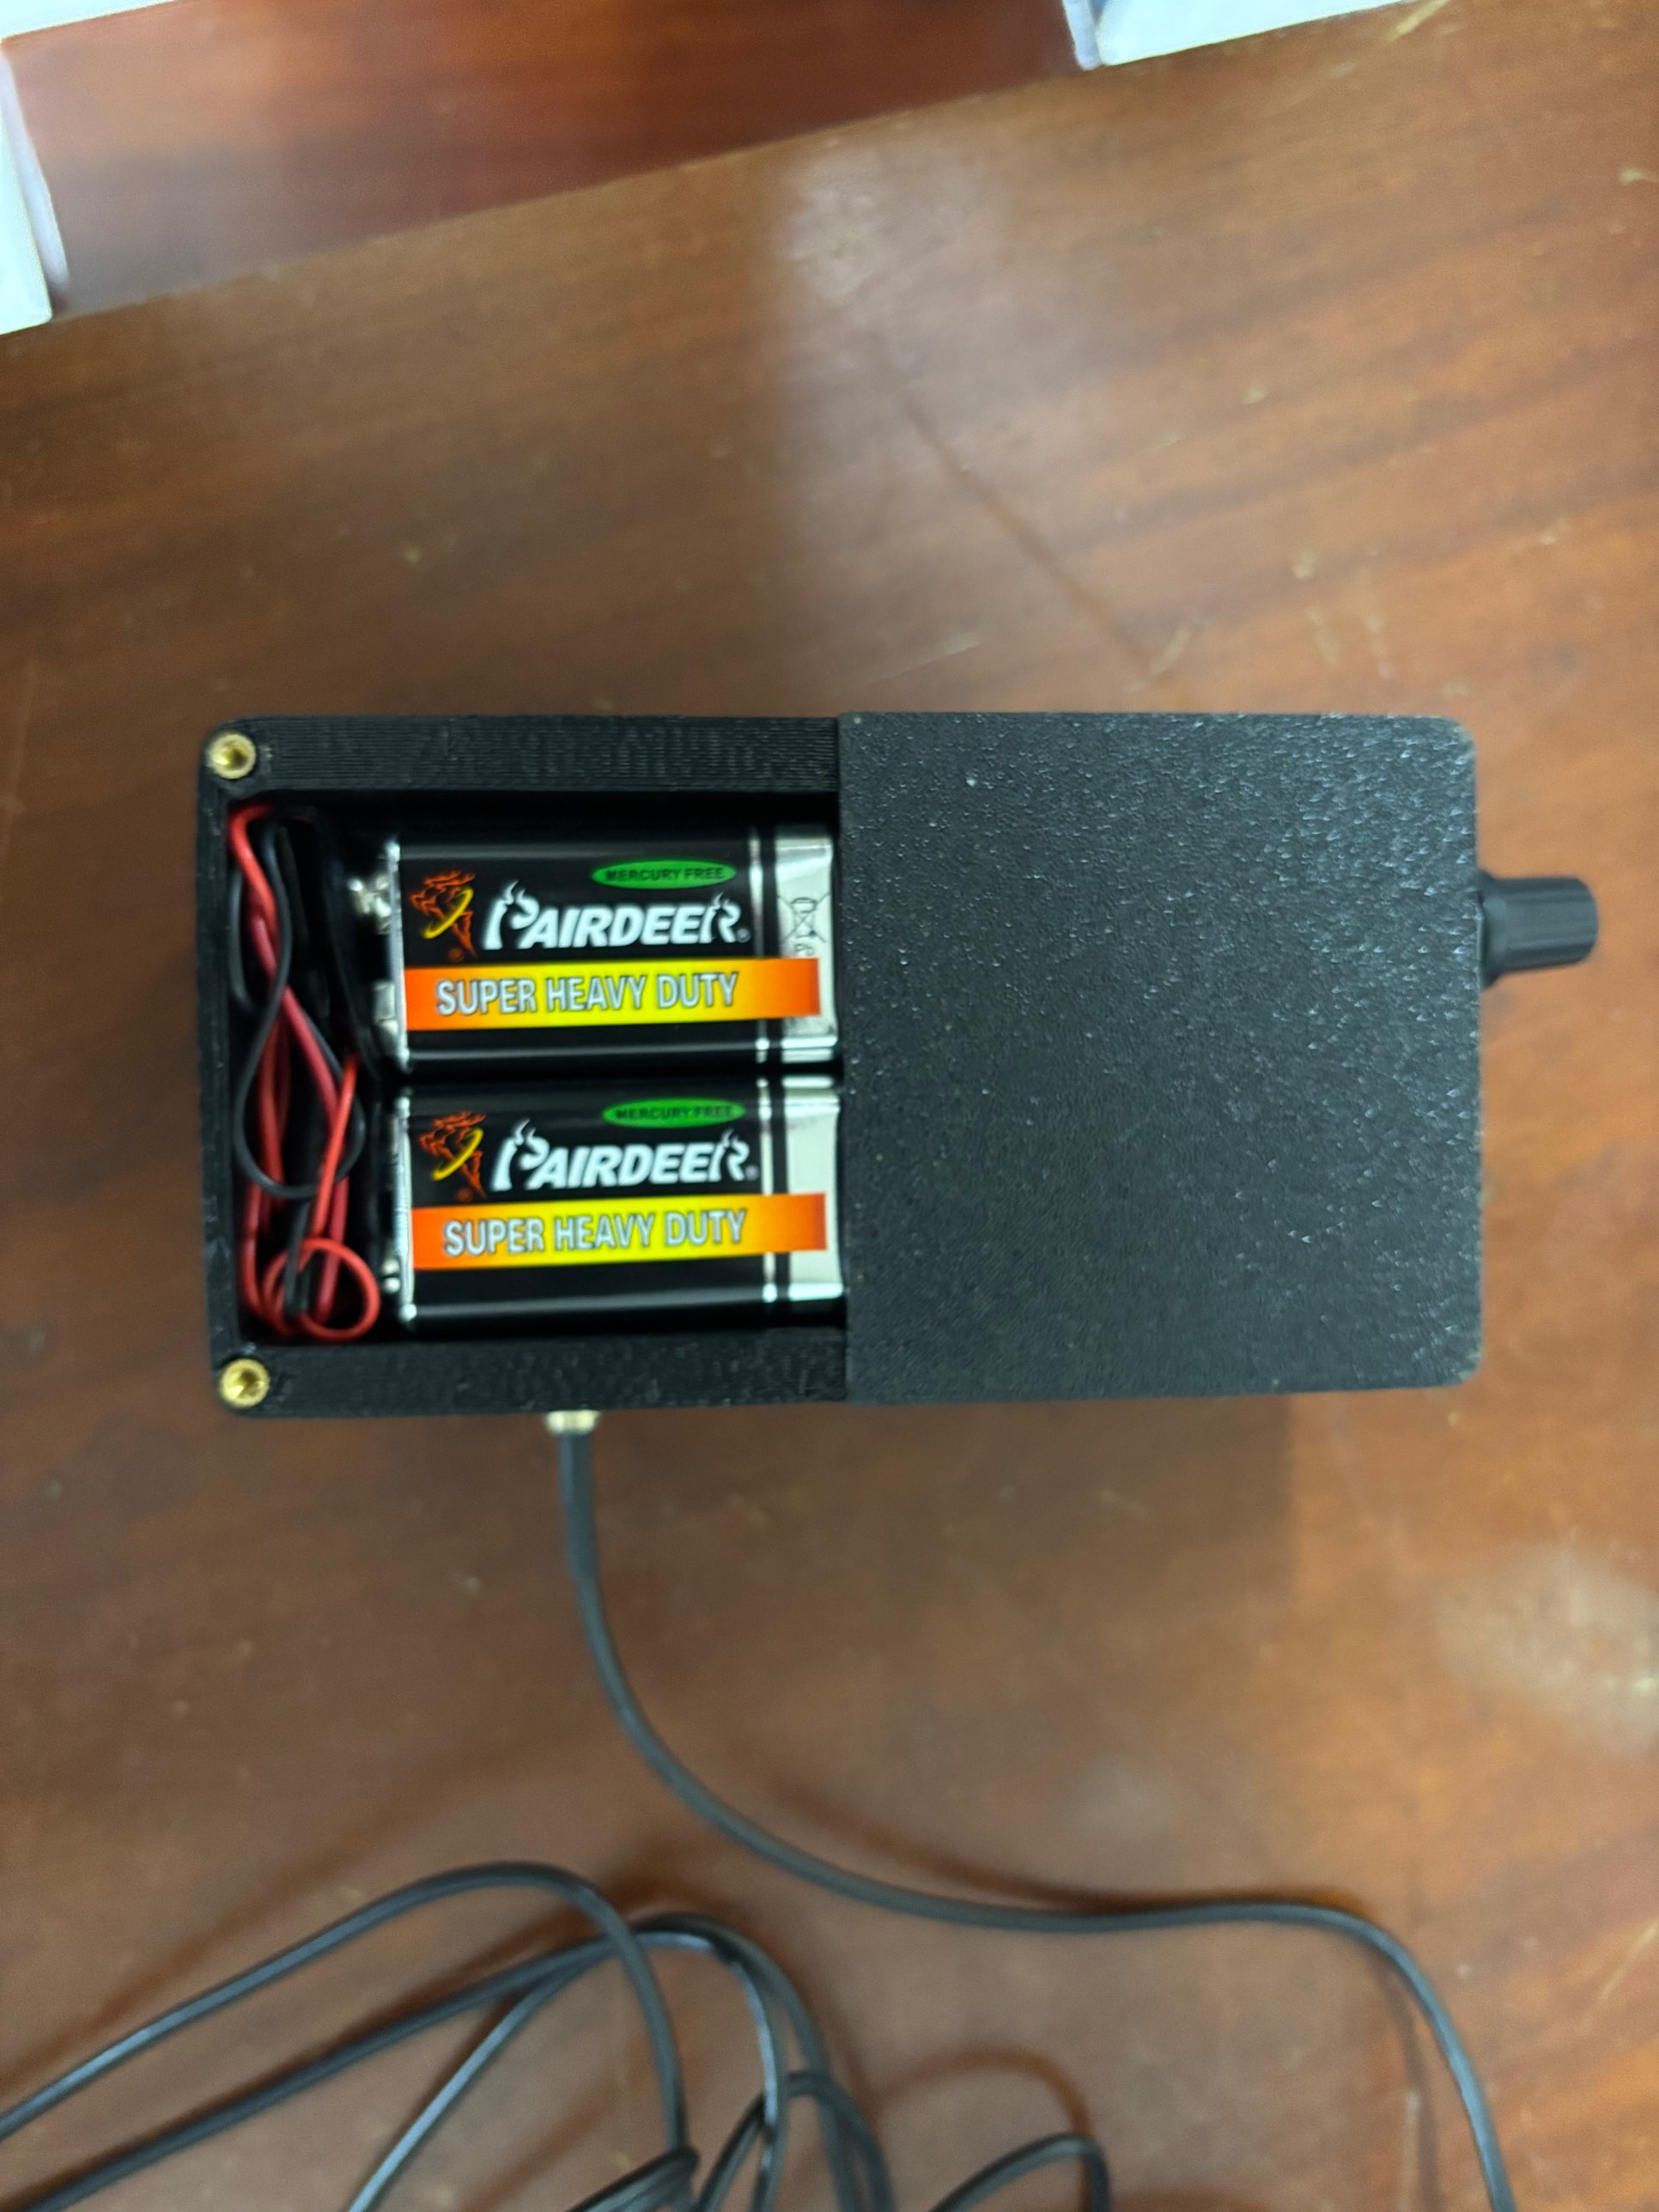
\includegraphics[width=\linewidth,height=4.2cm,keepaspectratio]{enclosure4.jpeg}\\
    {\small Battery compartment}
  \end{minipage}\hfill
  \begin{minipage}[t]{0.48\linewidth}
    \centering
    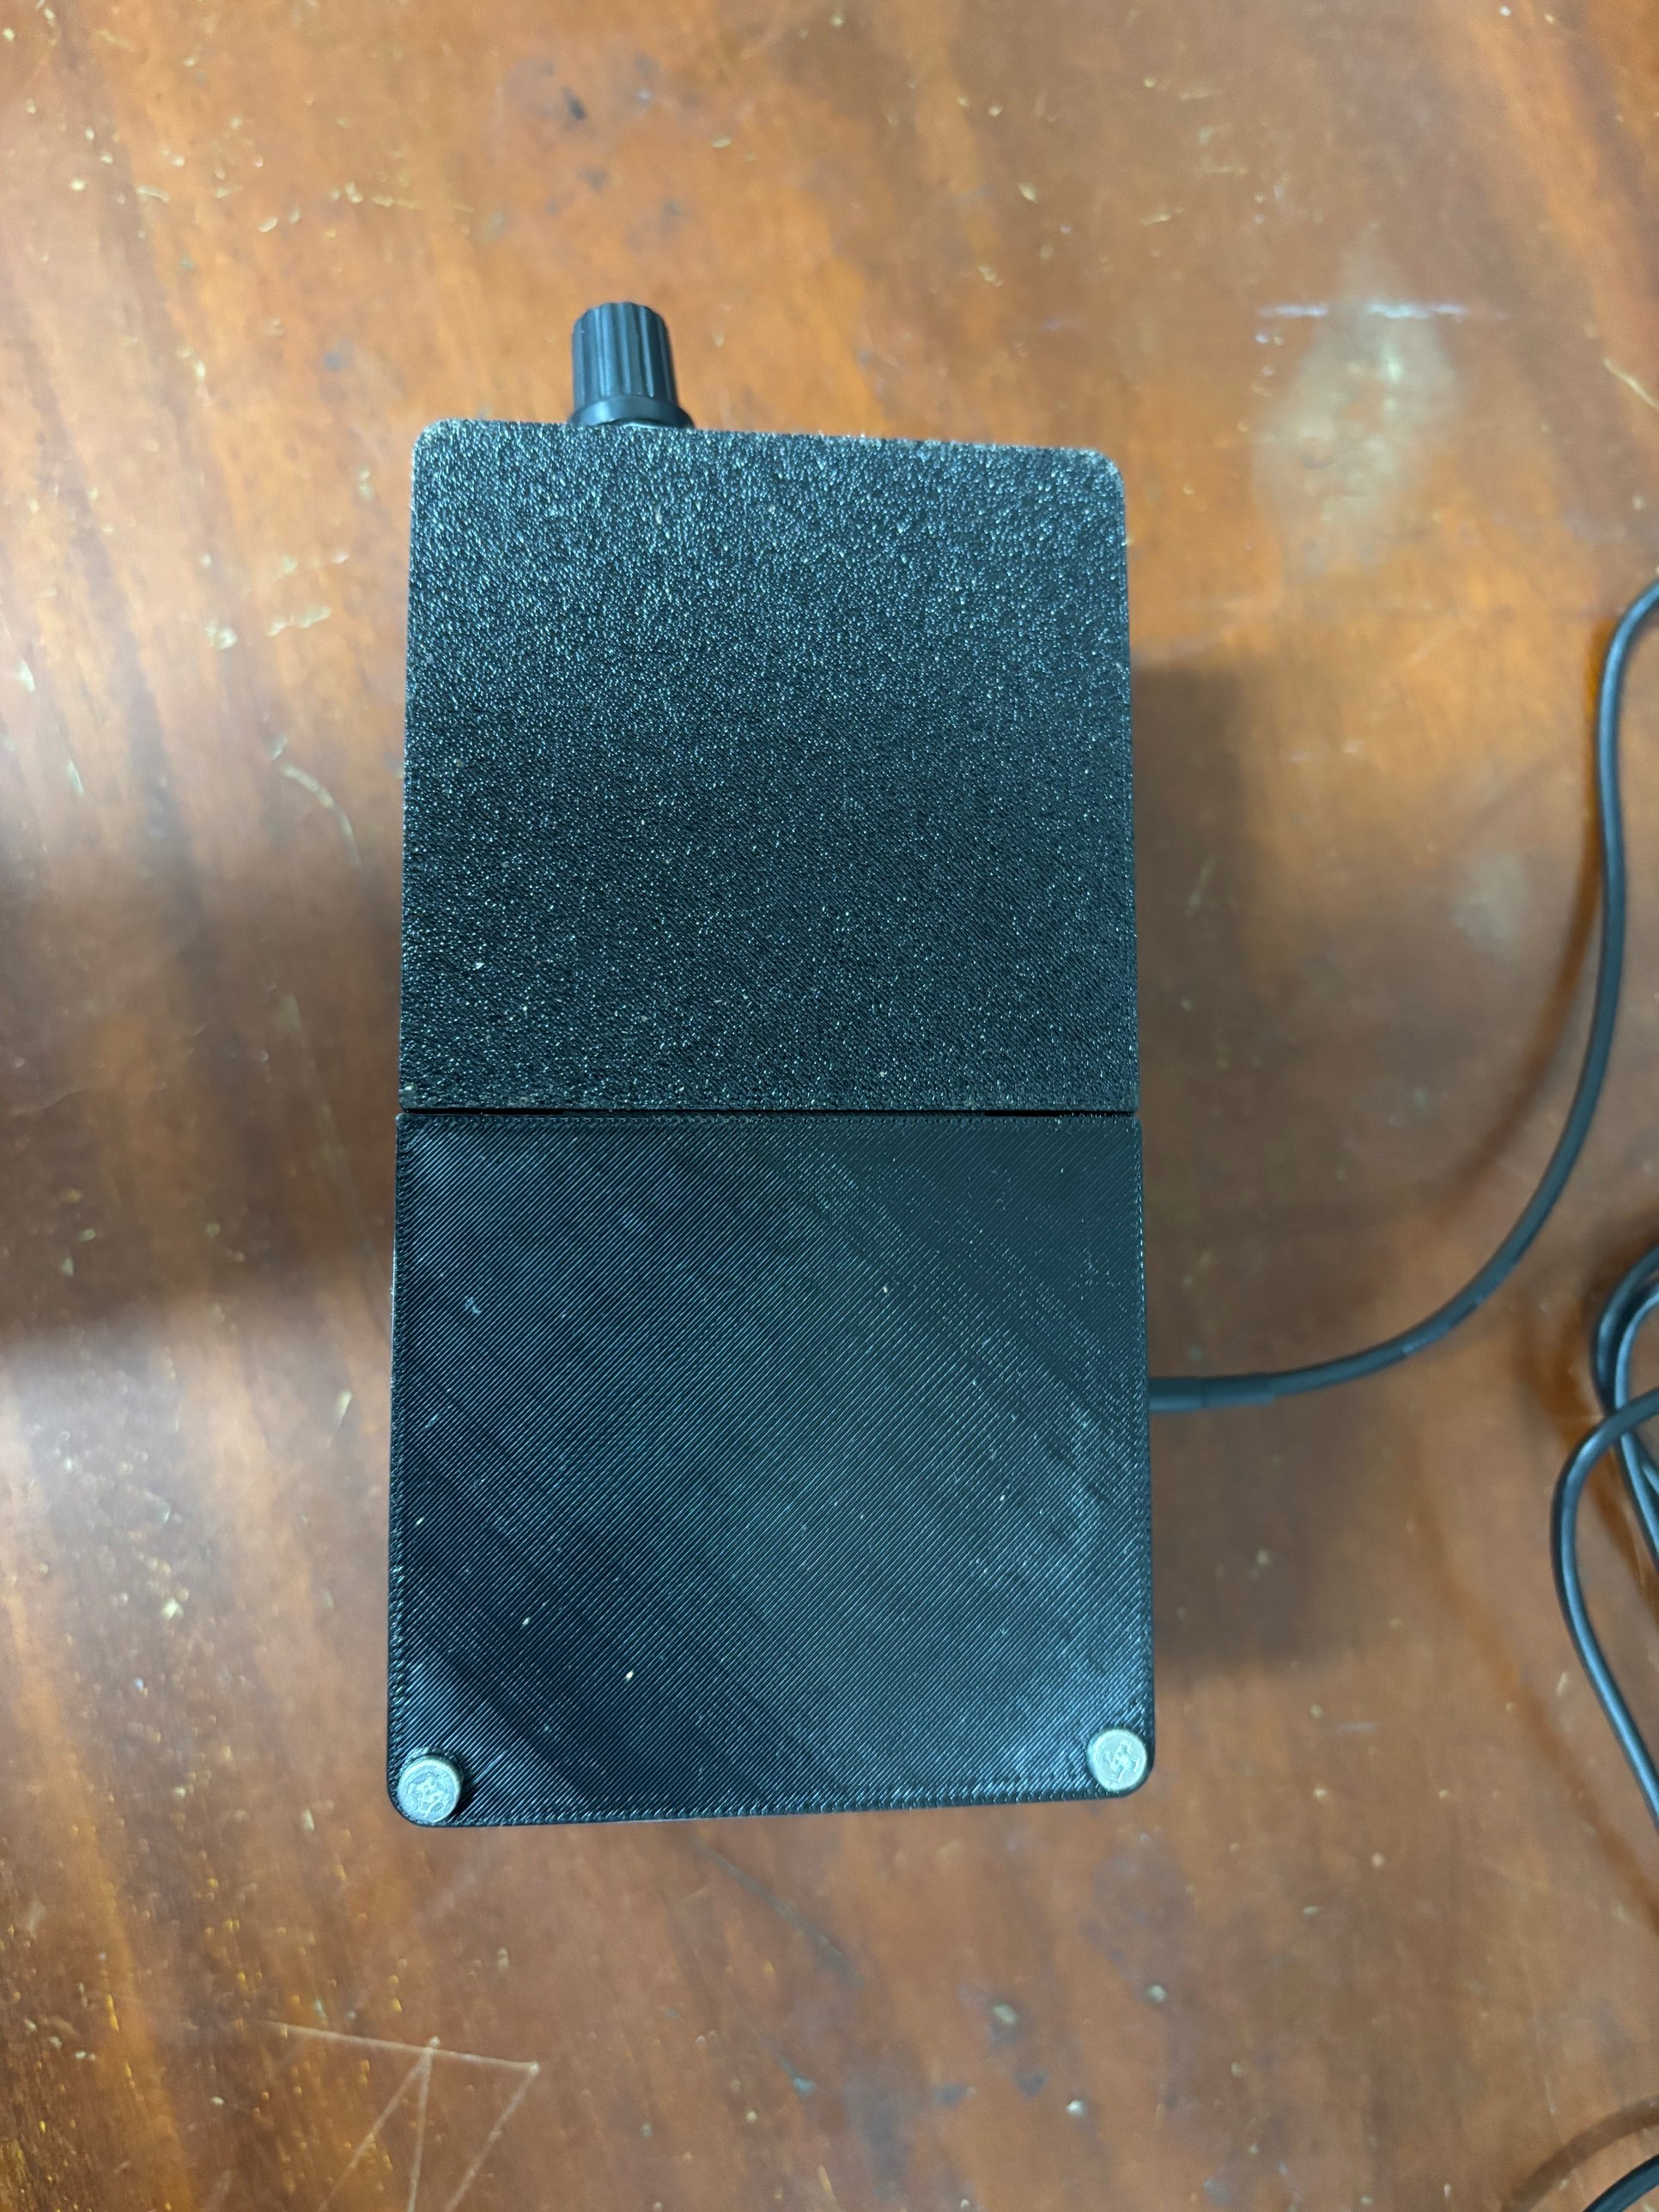
\includegraphics[width=\linewidth,height=4.2cm,keepaspectratio]{enclosure5.jpeg}\\
    {\small Closed battery compartment at the back}
  \end{minipage}

  \par\medskip
  \begin{minipage}[t]{0.48\linewidth}
    \centering
    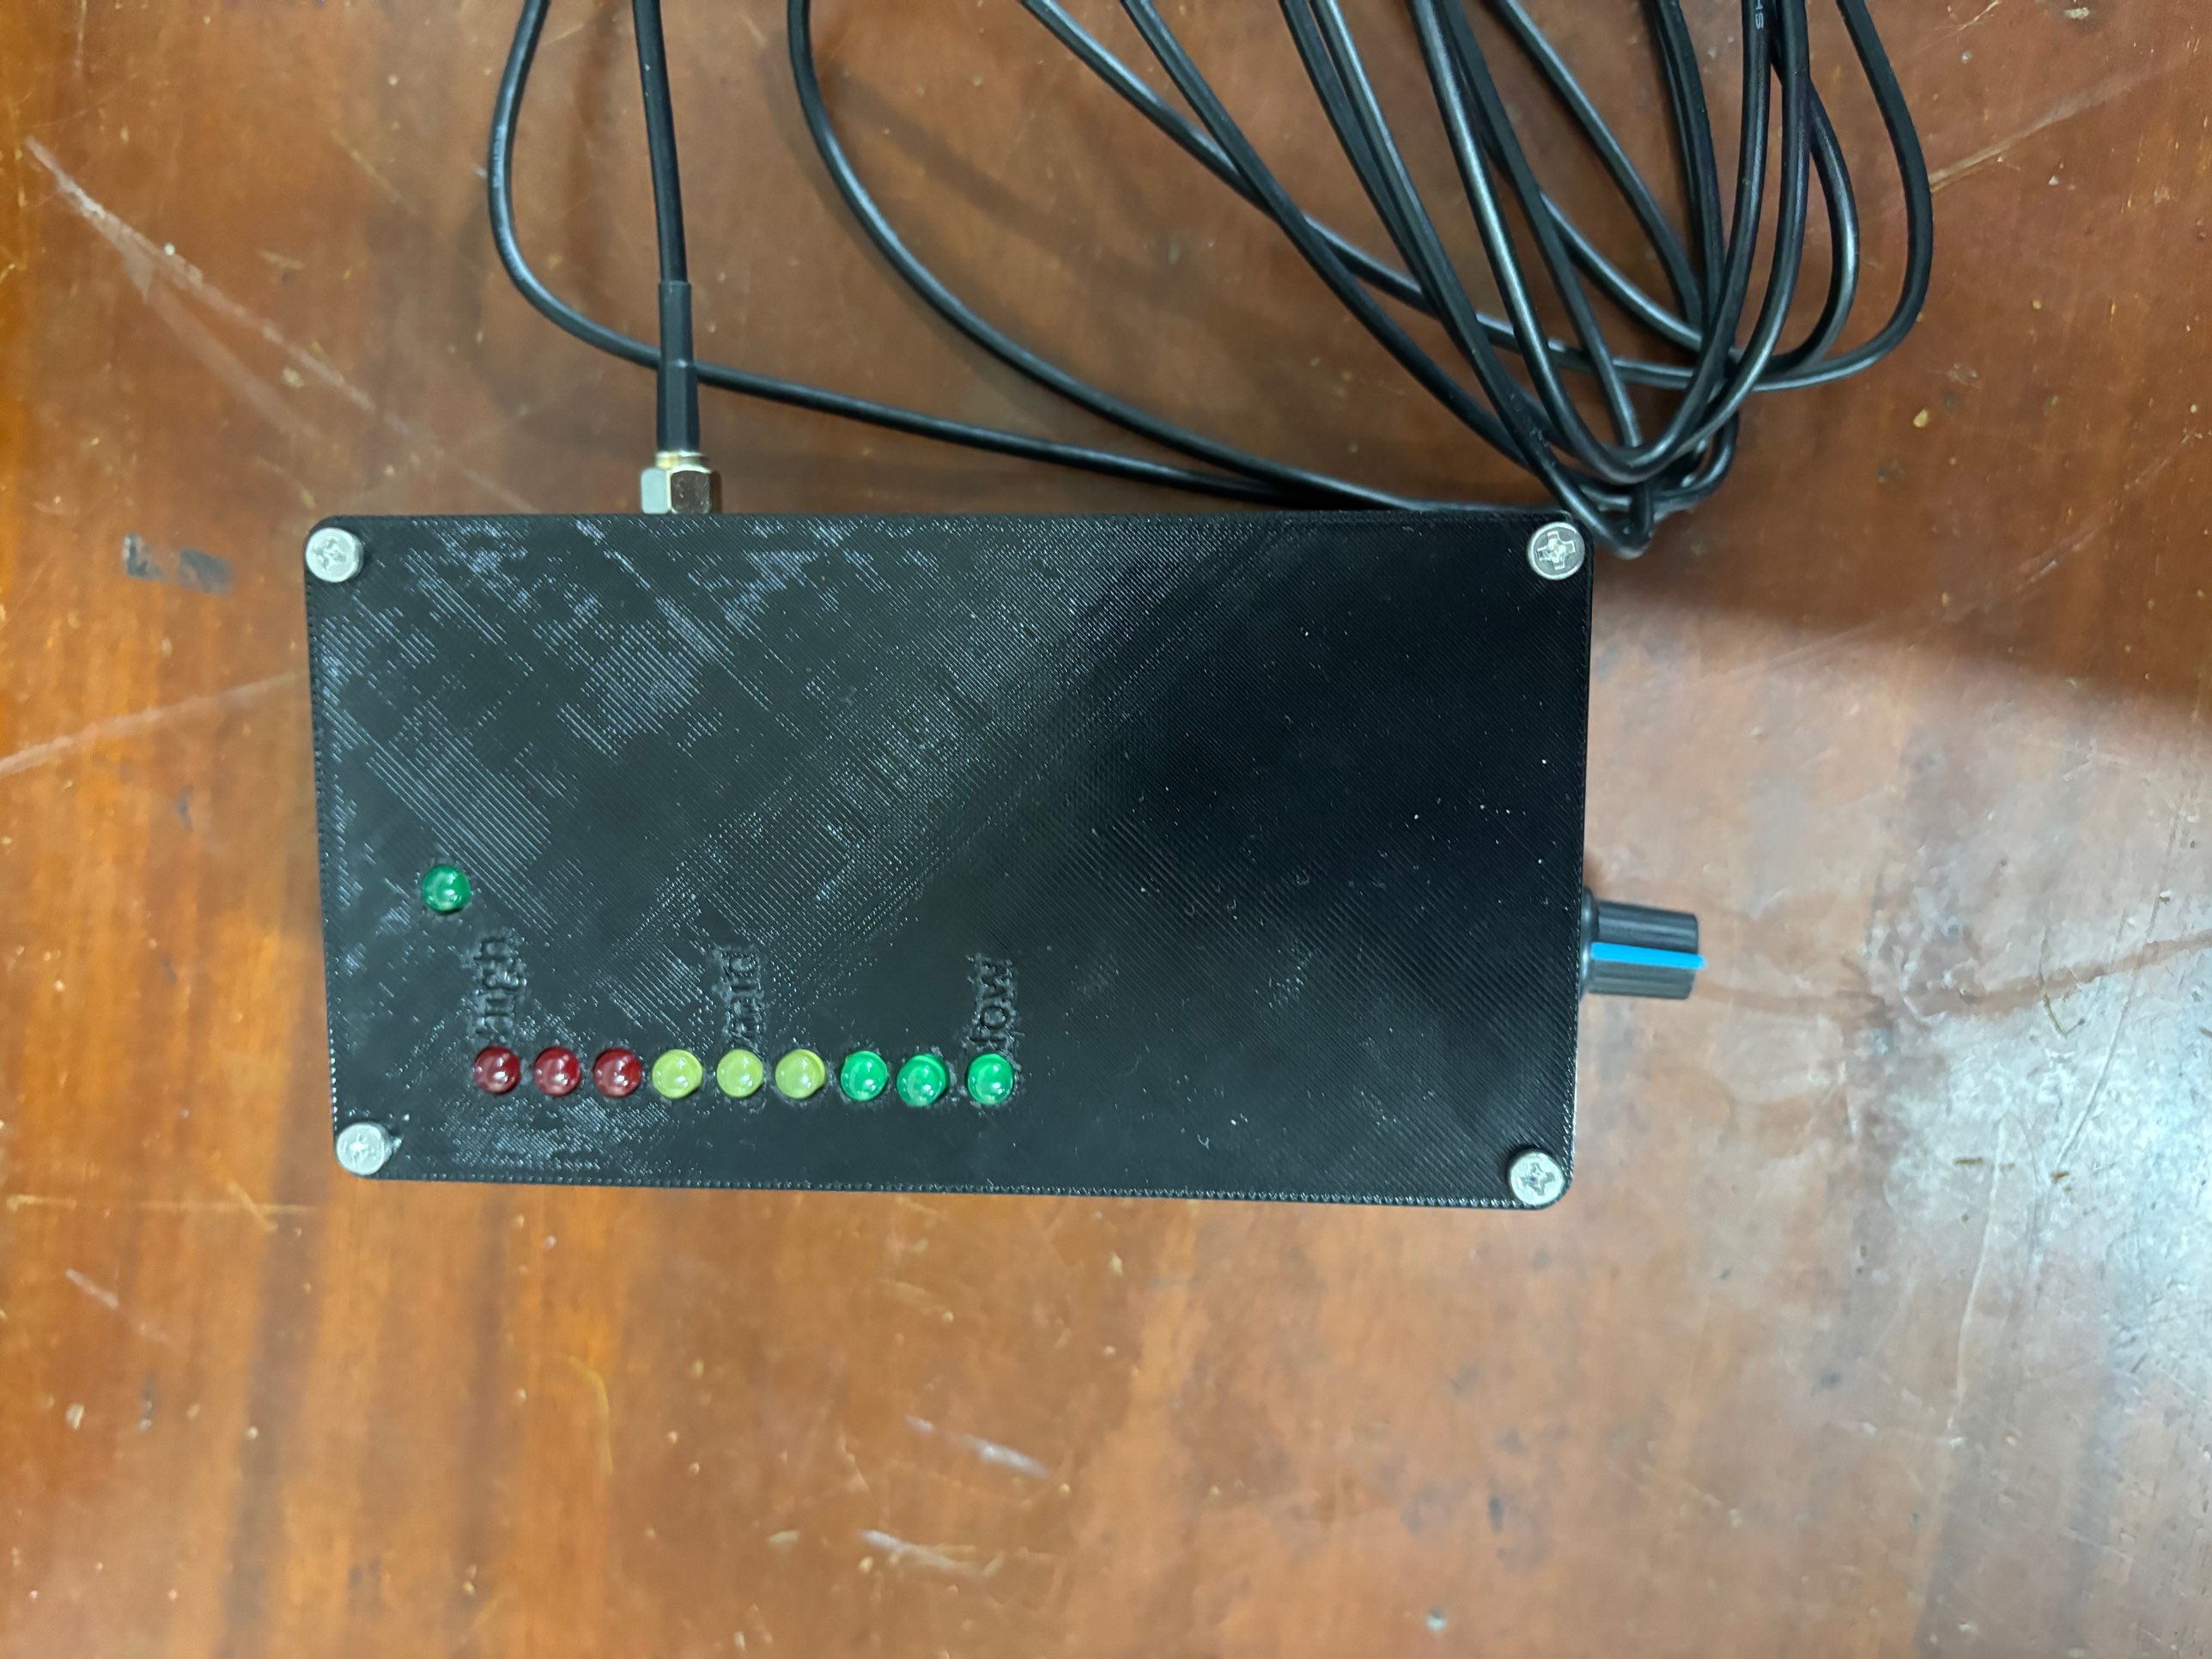
\includegraphics[width=\linewidth,height=4.2cm,keepaspectratio]{enclosure6.jpeg}\\
    {\small Front face with LED indicators}
  \end{minipage}\hfill
  \begin{minipage}[t]{0.48\linewidth}
    \centering
    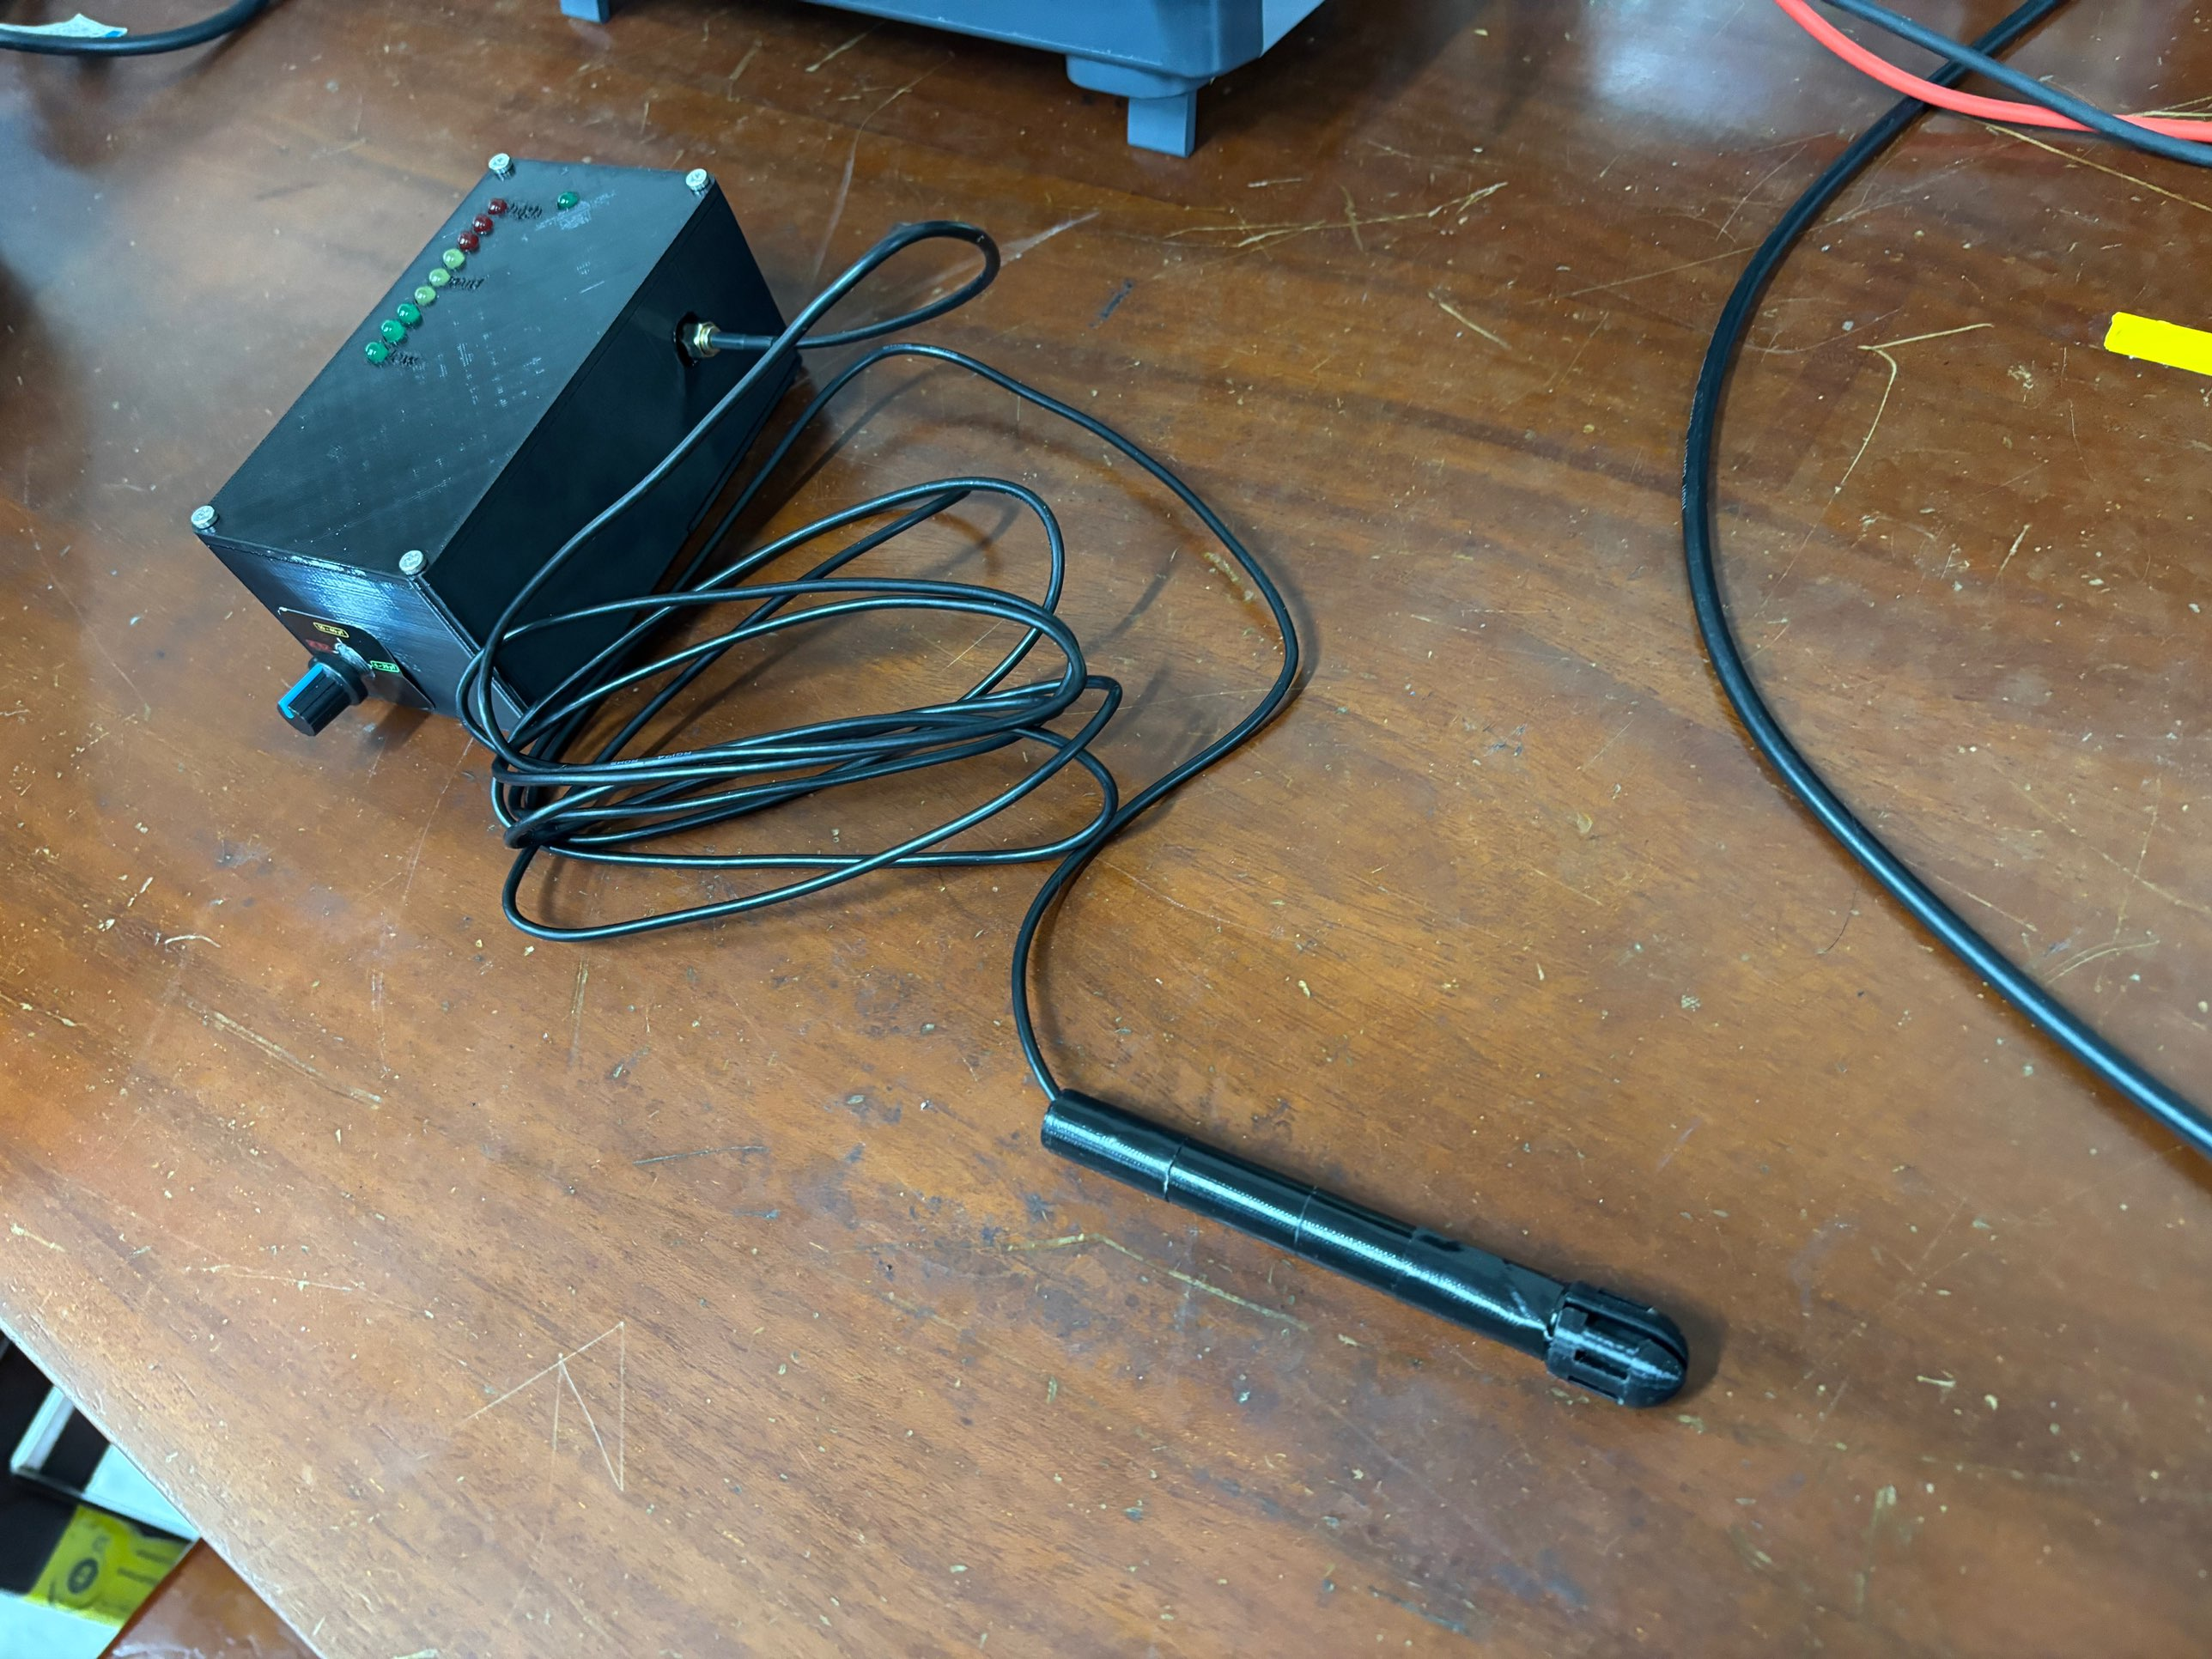
\includegraphics[width=\linewidth,height=4.2cm,keepaspectratio]{enclosure7.jpeg}\\
    {\small Probe connected to the main unit through coaxial}
  \end{minipage}
  \caption{Exterior and interior views of the detector enclosure.}
  \label{fig:enclosure-photos}
\end{figure}

% =====================================================================
% 6. Software Simulation and Hardware Testing
% =====================================================================
\section{Software Simulation and Hardware Testing}
\label{sec:testing}

The range of frequencies that this device is allowed to measure was determined through simulation in LTspice~\cite{ltspice} and then verified. We simulated both the frequency response and the complete operation of the device using the LTspice schematic in Figure~\ref{fig:ltspice_schematic}. The resulting frequency response is shown in Figure~\ref{fig:freq_response}.

\begin{figure}[H]
  \centering
  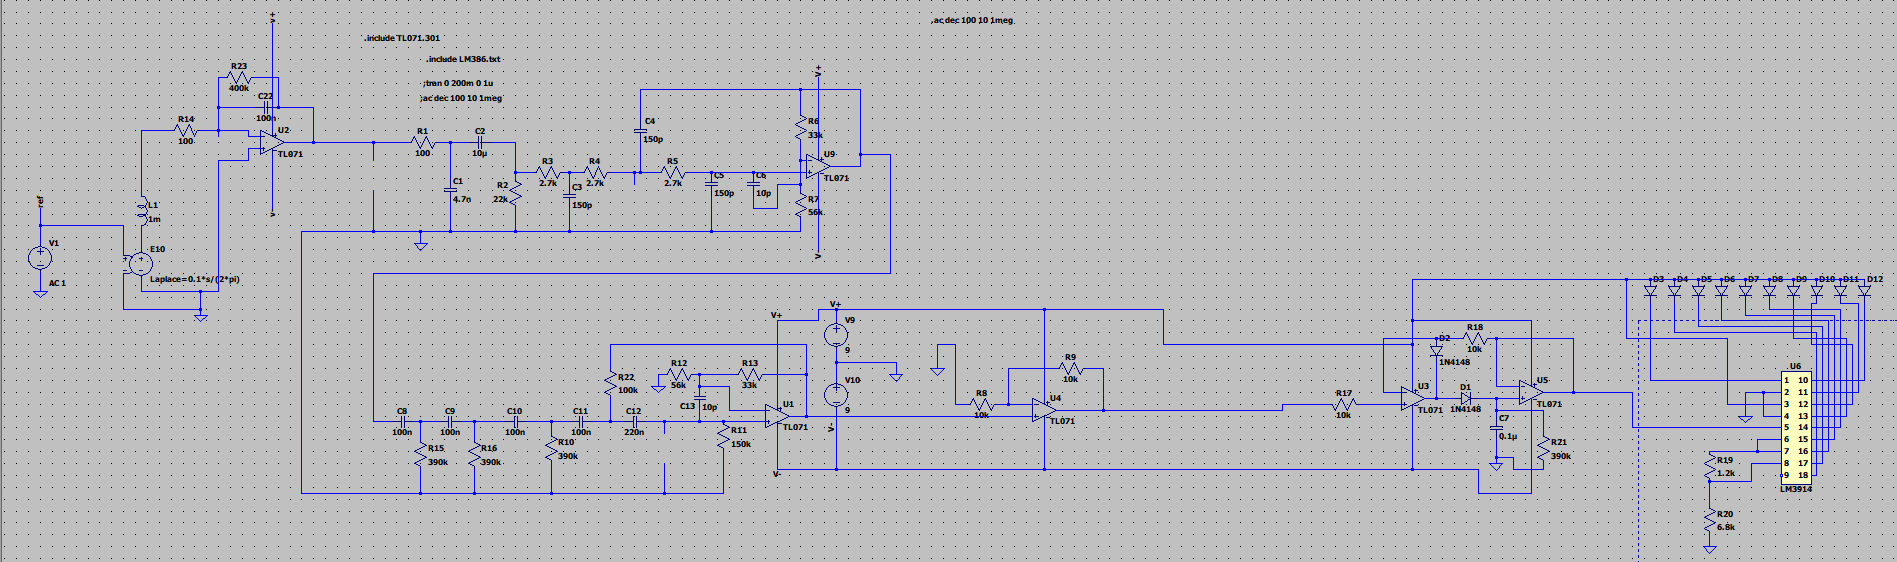
\includegraphics[angle=90,width=\linewidth,height=0.8\textheight,keepaspectratio]{image_3.png}
  \caption{LTspice schematic of the complete circuit.}
  \label{fig:ltspice_schematic}
\end{figure}

\begin{figure}[H]
  \centering
  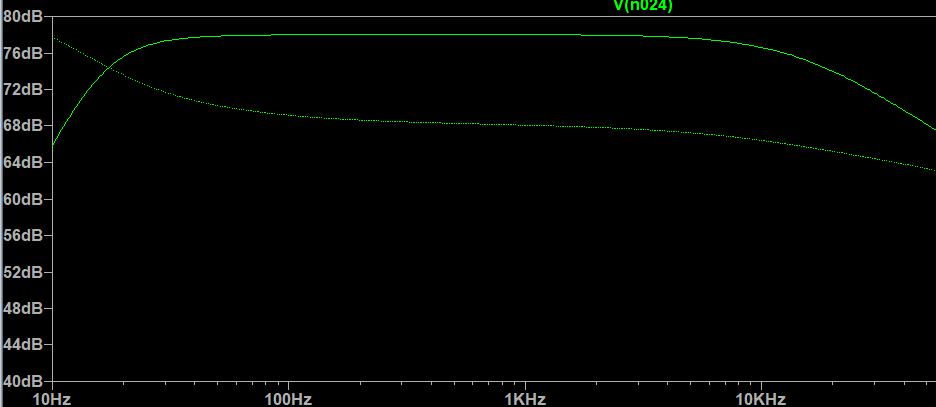
\includegraphics[width=\linewidth,height=5.8cm,keepaspectratio]{freq_response.png}
  \caption{LTspice frequency response (AC analysis) of the output node, showing the measurable frequency range of the device.}
  \label{fig:freq_response}
\end{figure}

To verify the actual working mechanism of the device, we needed to generate a magnetic field of known magnitude, so that we could check whether the corresponding LED lights up according to the strength of the magnetic field sensed by the probe. For this purpose we built a verifier circuit, which works according to the fundamentals of electromagnetics. A transconductance amplifier drives a coil, and the amplifier input is supplied by a signal generator. The AC current through the coil is measured by connecting a \SI{1}{\ohm} resistor in series with the coil. The voltage across this resistor is then numerically equal to the current driven through the coil. The test bench is shown in Figure~\ref{fig:test_bench}.

\begin{figure}[H]
  \centering
  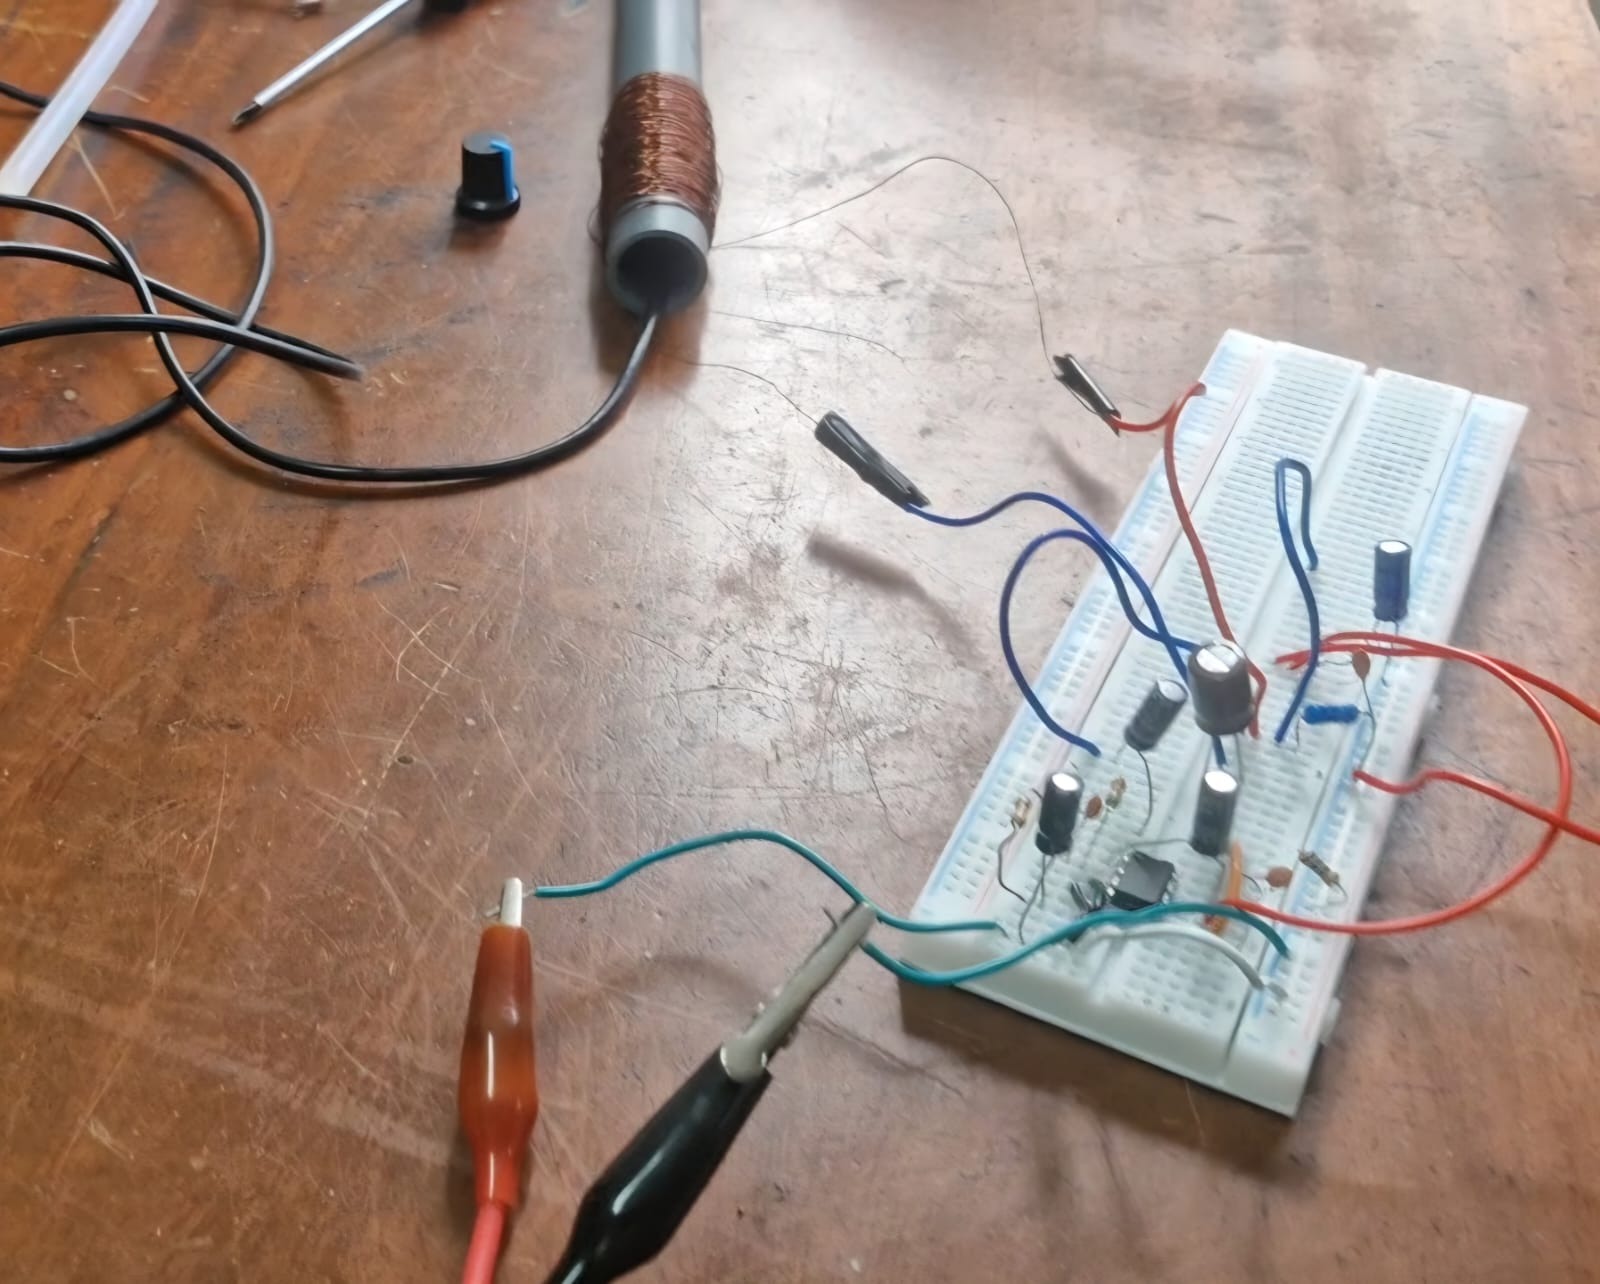
\includegraphics[width=\linewidth,height=6cm,keepaspectratio]{test_bench.jpeg}
  \caption{Test bench of the verifier circuit.}
  \label{fig:test_bench}
\end{figure}

Since a gauss meter was not available, we had to establish a mathematical relationship between the AC current through the coil and the resulting magnetic field. The flux density at the center of a finite solenoid of $N$ turns, diameter $D$ and winding length $\ell$ carrying a current $I$ is given by~\cite{griffiths2013}
\begin{equation}
  B = \frac{\mu_0 N I}{\sqrt{\ell^{2} + D^{2}}}.
  \label{eq:solenoid_general}
\end{equation}
For the coil used in testing ($N = 200$, $D = \SI{20}{\milli\meter}$, $\ell = \SI{50}{\milli\meter}$), Equation~\ref{eq:solenoid_general} gives
\begin{equation}
  B = \frac{4\pi\times10^{-7}\times 200\; I}{\sqrt{0.05^{2} + 0.02^{2}}}
    \approx 4.667\times10^{-3}\, I \quad \text{(T)},
\end{equation}
with $I$ in amperes. Because the current is sensed across the \SI{1}{\ohm} resistor, the voltage across it in millivolts equals the coil current in milliamperes, so
\begin{equation}
  \boxed{B\,[\mu\mathrm{T}] \approx 4.667 \times V_{\mathrm{check}}\,[\mathrm{mV}]}
  \label{eq:final_uT_mV}
\end{equation}
Each millivolt measured across the \SI{1}{\ohm} resistor therefore corresponds to a flux density of about \SI{4.667}{\micro\tesla} at the center of the coil.

For each of the three range settings, the probe was placed at the center of the coil and the coil current was increased slowly from zero. The current was noted when the lowest LED (LED~1) first lit and when the highest LED (LED~9) first lit, and the corresponding field was calculated using a rounded factor of \SI{4.6}{\micro\tesla} per \si{\milli\ampere}. This factor is about 1.4\,\% lower than the value in Equation~\ref{eq:final_uT_mV}, which is small compared with the step between adjacent LEDs. The results, taken at \SI{100}{\hertz}, are listed in Table~\ref{tab:measurements}.

\begin{table}[H]
  \centering
  \caption{Coil current and field at which the lowest and highest LEDs lit, for each range setting.}
  \label{tab:measurements}
  \small
  \begin{tabular}{@{}lccc@{}}
    \toprule
    Range setting & LED & Coil current (mA) & Field, $4.6\times I$ (\si{\micro\tesla}) \\
    \midrule
    \SIrange{5}{25}{\micro\tesla}  & 1 & 1.1  & 5.1  \\
                                   & 9 & 5.5  & 25.3 \\
    \SIrange{10}{40}{\micro\tesla} & 1 & 2.2  & 10.1 \\
                                   & 9 & 8.5  & 39.1 \\
    \SIrange{20}{90}{\micro\tesla} & 1 & 5.0  & 23.0 \\
                                   & 9 & 20.0 & 92.0 \\
    \bottomrule
  \end{tabular}
\end{table}

% =====================================================================
% 7. Conclusion & Future Works
% =====================================================================
\section{Conclusion \& Future Works}
\label{sec:conclusion}

\subsection{Conclusion}

The developed device is capable of detecting minor-scale AC magnetic leakages in the range of \SIrange{5}{90}{\micro\tesla}. Within this range, it provides a reliable indication of stray magnetic fields emitted by components such as inductors, transformers, small motors and current-carrying PCB traces. Although the device is primarily designed for this range, magnetic fields above \SI{90}{\micro\tesla} can still be detected, though not measured accurately, since the output saturates beyond the design limit.

\subsection{Future Works}

\subsubsection{Hardware Improvements}

\begin{itemize}
  \item \textbf{Extended measurement range:} The range can be extended up to \SI{500}{\micro\tesla} by increasing the supply voltage and reconfiguring the resistors of the non-inverting amplifier stage.
  \item \textbf{Quantitative readout:} An LCD display module can be added so the device outputs the actual strength of the measured magnetic field instead of only an indication of its presence.
\end{itemize}

\subsubsection{Potential Applications}

The \SIrange{5}{90}{\micro\tesla} range is relevant to many practical scenarios in electronics design and maintenance:

\begin{enumerate}
  \item \textbf{Protecting navigation and sensor accuracy:}
  \begin{itemize}
    \item \textit{Preventing compass and drone drift:} Digital magnetometers in smartphones, drones and autonomous robots rely on Earth's weak field ($\approx\SI{40}{\micro\tesla}$) to determine heading. A stray leakage of only \SIrange{5}{20}{\micro\tesla} from a nearby PCB trace or battery wire can introduce significant heading errors.
    \item \textit{Avoiding false Hall-effect triggers:} Magnetic sensors used for lid closure, wheel rotation or switch position detection can be falsely triggered by stray fields from nearby motors or inductors. Measuring background leakage helps prevent this.
  \end{itemize}

  \item \textbf{Ensuring electromagnetic compatibility (EMC):}
  \begin{itemize}
    \item \textit{Stopping internal crosstalk:} On compact boards, unshielded inductors can induce noise into adjacent audio lines, ADCs or RF circuits. Mapping fields in this range helps engineers place sensitive components at safe distances.
    \item \textit{Validating shielding and layout:} The device allows designers to verify whether shielded inductors, mu-metal sheets or improved PCB trace routing reduce stray flux to acceptable levels before mass production.
  \end{itemize}

  \item \textbf{Predictive maintenance and diagnostics:}
  \begin{itemize}
    \item \textit{Spotting component degradation early:} A sudden change in the stray magnetic signature of a small motor or transformer often indicates worn bearings, shorted turns or core saturation well before complete failure.
    \item \textit{Verifying power flow non-invasively:} Measuring the magnetic field around a PCB trace or wire lets technicians confirm current flow without cutting traces or breaking the circuit.
  \end{itemize}

  \item \textbf{Safety and regulatory compliance:}
  \begin{itemize}
    \item \textit{Meeting exposure and medical device standards:} Fields of this strength are below the public exposure limits at mains frequency, but bodies such as ICNIRP~\cite{icnirp2010} set frequency-dependent limits that become lower at higher frequencies. Implantable medical devices such as pacemakers also require clear magnetic exclusion zones around everyday electronics, which this device can help to identify.
  \end{itemize}
\end{enumerate}

Overall, with the proposed range extension and digital readout, the device can evolve from a basic leakage detector into a practical low-cost tool for EMC debugging, sensor protection, diagnostics and safety screening.

% =====================================================================
% 8. Contribution of Group Members
% =====================================================================
\section{Contribution of Group Members}
\label{sec:contributions}

The contributions of the four group members are summarized in Table~\ref{tab:group-contributions}.

\begin{table}[H]
  \centering
  \caption{Contributions of the group members.}
  \label{tab:group-contributions}
  \begin{tabular}{@{}p{0.38\linewidth}@{\hspace{4pt}}p{0.57\linewidth}@{}}
    \toprule
    Group member & Contribution \\
    \midrule
    Kumarasingha K. A. D. V. & Leading the team, PCB Design, Schematic Design, Component Selection \\
    Rathnasiri W. D. D. S. V. & PCB Design, Schematic Design, Component Selection \\
    Wickramarathna M. P. & Enclosure Design, Schematic Design, Component Selection \\
    Wijerathna N. A. C. M. & Enclosure Design, Schematic Design, Component Selection \\
    \bottomrule
  \end{tabular}
\end{table}

% =====================================================================
% Acknowledgment & Bibliography
% =====================================================================
\section*{Acknowledgment}
The team would like to acknowledge the coordination and guidance of Dr. Sampath Perera as the course coordinator. They further acknowledge the valuable advice of Dr. Upeka Premaratne and Mr. Kavishka Abeywardana. The support of all the laboratory assistants and technical officers, and the laboratory facilities of the university are also appreciated.

\bibliographystyle{IEEEtranN}
\bibliography{references}

\end{document}
